\documentclass{amsart}

\usepackage[T1]{fontenc}
\usepackage{amsmath, amsfonts, amssymb, amsthm, mathrsfs, wasysym, graphics, graphicx, xcolor, url, hyperref, hypcap, xargs, multicol, pdflscape, multirow, hvfloat, array, ae, aecompl, pifont, mathtools, a4wide, float, blkarray, overpic, nicefrac}
\usepackage[shortlabels, inline]{enumitem}%shortlabels to have same syntax as enumerate package, inline gives inline option with *
\usepackage{bbm}%allows for \mathbbm{1}
\usepackage[noabbrev,capitalise]{cleveref}
\usepackage[normalem]{ulem}
\usepackage{marginnote}
\hypersetup{colorlinks=true, citecolor=darkblue, linkcolor=darkblue}
\usepackage[all]{xy}
\usepackage{tikz}
\usepackage{tikz-cd}
%\usepackage{tkz-graph}
\usetikzlibrary{trees, decorations, decorations.pathmorphing, decorations.markings, decorations.shapes, shapes, arrows, matrix, calc, fit, intersections, patterns, angles}
\graphicspath{{figures/}{figures/diagonals/}{figures/walks/}{figures/tubes/}{figures/blocks/}}
\makeatletter\def\input@path{{figures/}}\makeatother
\usepackage{caption}
\captionsetup{width=\textwidth}
\usepackage[export]{adjustbox}

%%%%%%%%%%%%%%%%%%%%%%%%%%%%%%%%%%%%%%

% STANDARD

% theorems
\newtheorem{theorem}{Theorem}[section]
\newtheorem{corollary}[theorem]{Corollary}
\newtheorem{proposition}[theorem]{Proposition}
\newtheorem{lemma}[theorem]{Lemma}
\newtheorem{conjecture}[theorem]{Conjecture}
\newtheorem*{theorem*}{Theorem}%[section]

\theoremstyle{definition}
\newtheorem{definition}[theorem]{Definition}
\newtheorem{example}[theorem]{Example}
\newtheorem{remark}[theorem]{Remark}
\newtheorem{question}[theorem]{Question}
\newtheorem{notation}[theorem]{Notation}
\newtheorem{assumption}[theorem]{Assumption}
\newtheorem{convention}[theorem]{Convention}

\crefname{equation}{Equation}{Equations}

% math special letters
\newcommand{\R}{\mathbb{R}} % reals
\newcommand{\Q}{\mathbb{Q}} % rationals
\newcommand{\N}{\mathbb{N}} % naturals
\newcommand{\Z}{\mathbb{Z}} % integers
\newcommand{\C}{\mathbb{C}} % complex
\newcommand{\I}{\mathbb{I}} % set of integers
\newcommand{\K}{k} % field
\newcommand{\bb}[1]{{\mathbb{#1}}} % mathbb letters
\newcommand{\f}[1]{{\mathfrak{#1}}} % mathfrak letters
\renewcommand{\c}[1]{{\mathcal{#1}}} % call letters
\renewcommand{\b}[1]{{\boldsymbol{#1}}} % bold letters
\newcommand{\h}{\widehat} % hat letters

% math commands
\newcommand{\set}[2]{\left\{ #1 \;\middle|\; #2 \right\}} % set notation
\newcommand{\bigset}[2]{\big\{ #1 \;\big|\; #2 \big\}} % big set notation
\newcommand{\Bigset}[2]{\Big\{ #1 \;\Big|\; #2 \Big\}} % Big set notation
\newcommand{\setangle}[2]{\left\langle #1 \;\middle|\; #2 \right\rangle} % set notation
\newcommand{\ssm}{\smallsetminus} % small set minus
\newcommand{\dotprod}[2]{\langle \, #1 \; | \; #2 \, \rangle} % dot product
\newcommand{\bigdotprod}[2]{\big\langle \, #1 \; \big| \; #2 \, \big\rangle} % dot product
\newcommand{\symdif}{\,\triangle\,} % symmetric difference
\newcommand{\one}{\mathbbm{1}} % the all one vector
\newcommandx{\ones}[1][1=n]{\one_{#1}} % the all one vector of length n
\newcommand{\eqdef}{\mbox{\,\raisebox{0.2ex}{\scriptsize\ensuremath{\mathrm:}}\ensuremath{=}\,}} % :=
\newcommand{\defeq}{\mbox{~\ensuremath{=}\raisebox{0.2ex}{\scriptsize\ensuremath{\mathrm:}} }} % =:
\newcommand{\simplex}{\triangle} % simplex
\renewcommand{\implies}{\Rightarrow} % imply sign
\newcommand{\transpose}[1]{{#1}^T} % transpose matrix
\newcommand{\truth}[1]{\left[ #1 \right]} % truth (kronecker delta)

% operators
\DeclareMathOperator{\conv}{conv} % convex hull
\DeclareMathOperator{\vect}{vect} % linear span
\DeclareMathOperator{\cone}{cone} % cone hull
\DeclareMathOperator{\colim}{colim} % colimit

% others
\newcommand{\ie}{\textit{i.e.}~} % id est
\newcommand{\eg}{\textit{e.g.}~} % exempli gratia
\newcommand{\Eg}{\textit{E.g.}~} % exempli gratia
\newcommand{\apriori}{\textit{a priori}} % a priori
\newcommand{\viceversa}{\textit{vice versa}} % vice versa
\newcommand{\versus}{\textit{vs.}~} % versus
\newcommand{\aka}{\textit{a.k.a.}~} % also known as
\newcommand{\perse}{\textit{per se}} % per se
\newcommand{\ordinal}{\textsuperscript{th}} % th for ordinals
\newcommand{\ordinalst}{\textsuperscript{st}} % st for ordinals
\definecolor{darkblue}{rgb}{0,0,0.7} % darkblue color
\definecolor{green}{RGB}{57,181,74} % green color
\definecolor{violet}{RGB}{147,39,143} % violet color
\newcommand{\red}{\color{red}} % red command
\newcommand{\blue}{\color{blue}} % blue command
\newcommand{\orange}{\color{orange}} % orange command
\newcommand{\green}{\color{green}} % green command
\newcommand{\darkblue}{\color{darkblue}} % darkblue command
\newcommand{\defn}[1]{\textsl{\darkblue #1}} % emphasis of a definition
\newcommand{\para}[1]{\medskip\noindent\uline{\textit{#1.}}} % paragraph
\renewcommand{\topfraction}{1} % possibility to have one page of pictures
\renewcommand{\bottomfraction}{1} % possibility to have one page of pictures
\newcommand{\shade}[1]{{\color{cyan} #1}}
\newcommand{\as}{{\scriptstyle \text{\rm !`}}} %Antischrieck
\tikzset{inner sep=0.4mm}

% marginal comments
\usepackage{todonotes}
\newcommand{\guillaume}[1]{\todo[color=orange!30]{#1 --- G.}}
\newcommand{\vincent}[1]{\todo[color=blue!30]{#1 \\ \hfill --- V.}}

% formating the part command
\makeatletter
\def\part{\@startsection{part}{1}%
\z@{.7\linespacing\@plus\linespacing}{.8\linespacing}%
{\LARGE\sffamily\centering}}
%\@addtoreset{section}{part}
\makeatother
\renewcommand{\thepart}{\Roman{part}}
%\renewcommand{\thesection}{\arabic{part}.\arabic{section}}

% formating the table of contents
\setcounter{tocdepth}{4}
\makeatletter
\def\l@section{\@tocline{1}{5pt}{0pc}{}{}}
\makeatother
\let\oldtocpart=\tocpart
\renewcommand{\tocpart}[2]{\sc\large\oldtocpart{#1}{#2}}
\let\oldtocsection=\tocsection
\renewcommand{\tocsection}[2]{\bf\oldtocsection{#1}{#2}}
\let\oldtocsubsubsection=\tocsubsubsection
\renewcommand{\tocsubsubsection}[2]{\quad\oldtocsubsubsection{#1}{#2}}

% drapeau européen
\usepackage{graphicx,calc}
\newlength\myheight
\newlength\mydepth
\settototalheight\myheight{Xygp}
\settodepth\mydepth{Xygp}
\setlength\fboxsep{0pt}
\newcommand*\inlinegraphics[1]{%
  \settototalheight\myheight{Xygp}%
  \settodepth\mydepth{Xygp}%
  \raisebox{-\mydepth}{\includegraphics[height=\myheight]{#1}}%
}

% SPECIFIC BLOCK GRAPH PERMUTREES

% COMBINATORICS

% decorations
\newcommandx{\Maple}[1][1=M]{#1} % maple tree
\newcommandx{\decoratedMaple}[1][1=\Maple]{\b{#1}} % maple tree
\newcommandx{\Graph}[1][1=G]{#1} % graph
\newcommandx{\decoratedGraph}[1][1=\Graph]{\b{#1}} % decorated graph
\newcommandx{\vertexSet}[1][1=V]{#1} %vertex set
\newcommandx{\edgeSet}[1][1=E]{#1} %edge set
\newcommand{\decoration}{\delta}
\newcommandx{\Up}[2][1=v, 2=\decoration]{\smash{\overline #2}(#1)} 
\newcommandx{\Down}[2][1=v, 2=\decoration]{\smash{\underline #2}(#1)} 
\newcommandx{\up}[1][1=v]{\overline{#1}} 
\newcommandx{\down}[1][1=v]{\underline{#1}} 
\newcommandx{\updown}[1][1=v]{\overline{\underline{#1}}} 
% source and target
\newcommandx{\so}[1][1=i]{\textsc{s}_{#1}} % source set
\newcommandx{\ta}[1][1=o]{\textsc{t}_{#1}} % target set
% spines
\newcommandx{\spine}[1][1=S]{#1} % spine
\newcommandx{\almostSpine}[1][1=S]{\smash{\widetilde{#1}}} % spine
\newcommandx{\spines}[1][1=\decoratedGraph]{\mathcal{S}(#1)} % set of spines
\newcommandx{\spinePoset}[1][1=\decoratedGraph]{\mathcal{P}_{#1}} % spine poset
\newcommand{\blossom}{^\text{\ding{96}}} % blossom
\newcommand{\labeling}{\lambda} % labels in blossoming trees
\newcommandx{\equivalenceSpines}[2][1=\decoratedGraph, 2=\decoratedGraph']{\equiv_{#1 \to #2}} % equivalence relation on spines
% nested complex
\newcommandx{\chunk}[1][1=C]{#1} % chunck
\newcommandx{\nested}[1][1=N]{#1} % nested set
\newcommand{\negNested}{\preceq} % negative nested
\newcommand{\posNested}{\succeq} % positive nested
\newcommand{\negDisjoint}{\perp} % negative disjoint
\newcommand{\posDisjoint}{\;\top\;} % positive disjoint
\newcommandx{\nestedComplex}[1][1=\decoratedGraph]{\mathcal{N}_{#1}} % nested complex
% maps
\newcommand{\spineToNested}{\mathsf{N}} % spine to nested set
\newcommand{\nestedToSpine}{\mathsf{S}} % nested set to spine
\newcommand{\partitionToSpine}{\mathsf{S}} % partition to spine
\newcommandx{\surjectionSpines}[2][1=\decoratedGraph, 2=\decoratedGraph']{\Phi_{#1 \to #2}} % spine to spine
\newcommand{\nodeSurj}[2]{\smash{n_{#1}^{#2}}} % node surjection
\newcommand{\arcSurj}[2]{\smash{\varepsilon_{#1}^{#2}}} % arc surjection
% insertion
\newcommand{\insertion}[2]{#1 \ll #2} % insertion

% GEOMETRY

% fans
\newcommand{\primalCone}{\mathsf{C}^\star} % primal cone
\newcommand{\normalCone}{\mathsf{C}} % normal cone
\newcommandx{\braidFan}[1][1=\Graph]{\mathcal{F}_{#1}} % braid fan
\newcommandx{\sylvesterFan}[1][1=\Graph]{\mathcal{T}_{#1}} % sylvester fan
\newcommandx{\graphicalFan}[1][1=\Graph]{\mathcal{G}_{#1}} % graphical fan
\newcommandx{\spineFan}[1][1=\decoratedGraph]{\mathcal{S}_{#1}} % spine fan
% polytopes
\newcommand{\polytope}[1]{\mathsf{#1}} % font polytopes
\newcommandx{\Perm}[2][1=\Graph,2=\weight]{\polytope{Perm}^{#2}_{#1}} % permutahedron
\newcommandx{\Asso}[2][1=\Graph,2=\weight]{\polytope{Asso}^{#2}_{#1}} % associahedron
\newcommandx{\Spin}[2][1=\decoratedGraph,2=\weight]{\polytope{Spin}^{#2}_{#1}} % spine polytope
\newcommandx{\Zono}[2][1=\Graph,2=\weight]{\mathsf{Zono}^{#2}_{#1}} % zonotope
\newcommandx{\point}[2][1=\spine,2=\weight]{\b{a}^{#2}_{#1}} % point
\newcommand{\weight}{\omega} % weight
\newcommandx{\boundary}[1][1=\pi]{\partial#1} % endpoints of a path
\newcommandx{\peaks}[1][1=\pi]{\wedge#1} % top of a path
\newcommandx{\valleys}[1][1=\pi]{\vee#1} % bottom of a path
\newcommandx{\Hyp}[1][1=\weight]{\mathbf{H}^{= #1}} % hyperplane
\newcommandx{\HS}[1][1=\weight]{\mathbf{H}^{\ge #1}} % halfspace
\newcommand{\monombinom}[1]{\big\{\!\begin{smallmatrix} #1 \\ 2 \end{smallmatrix}\!\big\}}

%%%%%%%%%%%%%%%%%%%%%%%%%%%%%%%%%%%%%%

\title{Spine polytopes}

\author{Guillaume Laplante-Anfossi}
\address[Guillaume Laplante-Anfossi]{Universit\'e Sorbonne Paris Nord, Laboratoire Analyse, G\'eom\'etrie et Applications, CNRS, UMR 7539, F-93430 Villetaneuse, France}
\email{laplante-anfossi@math.univ-paris13.fr}
\urladdr{\url{https://www.math.univ-paris13.fr/~laplante-anfossi/}}

\author{Vincent Pilaud}
\address[Vincent Pilaud]{CNRS \& LIX, \'Ecole Polytechnique, Palaiseau}
\email{vincent.pilaud@lix.polytechnique.fr}
\urladdr{\url{http://www.lix.polytechnique.fr/~pilaud/}}

%\date{\today}

\subjclass[2010]{Primary 52B11; Secondary 18M70} 

%\keywords{Polytopes...}

\thanks{The first author was supported by the European Union's Horizon 2020 research and innovation program under the Marie Sklodowska-Curie grant agreement No 754362 \inlinegraphics{EU.png}, by the Natural Sciences and Engineering Research Council of Canada (NSERC) and by the ANR-20-CE40-0016 Higher Algebra, Geometry and Topology. The second author is supported by the French ANR grants CAPPS~17\,CE40\,0018, and CHARMS~19\,CE40\,0017.}

%%%%%%%%%%%%%%%%%%%%%%%%%%%%%%%%%%%%%%
%%%%%%%%%%%%%%%%%%%%%%%%%%%%%%%%%%%%%%%

\begin{document}

\begin{abstract}
TBC
\end{abstract}

\maketitle

\tableofcontents

%%%%%%%%%%%%%%%%%%%%%%%%%%%%%%%%%%%%%%%
%%%%%%%%%%%%%%%%%%%%%%%%%%%%%%%%%%%%%%%

\newpage
\section*{Introduction}

Common generalization of \cite{Pilaud-signedTreeAssociahedraFPSAC, LangePilaud, PilaudPons-permutrees, Laplante-diagonalOperahedra}.
It is the maximal generalization, according to \cite{Pilaud-removahedra}.

\guillaume{dioperads and string topology}
\guillaume{our dioperad might be initial in some operadic / Feynman / moment category}
\vincent{Block graphs already appear in our context: exactly the graphs whose graphical zonotope is simple, and exactly the graphs whose graph associahedra are removahedra. Btw, this is already a reason for the construction not working beyond block graphs.}
\vincent{Line graphs of trees are exactly claw-free block graphs.}

%%%%%%%%%%%%%%%%%%%%%%%%%%%%%%%%%%%%%%%
%%%%%%%%%%%%%%%%%%%%%%%%%%%%%%%%%%%%%%%

\newpage
\section{Combinatorics: Spine Poset and Nested Complex}
\label{sec:combinatorics}

This section is dedicated to the combinatorics of spines on decorated block graphs.

%%%%%%%%%%%%%%%%%%%%%%%%%%%%%%%%%%%%%%%

\subsection{Maple trees and block graphs}
\label{subsec:MapleTreesBlockGraphs}

We start by defining the ground sets of our constructions.
We will use both maple trees and block graphs, which essentially encode the same information.

\begin{definition}
  A \defn{maple tree} is a tree whose vertices are properly colored (\ie no monochromatic edge) in red and blue such that all leaves are red.
  \vincent{should blue be gray?}
  The \defn{tapping} of a maple tree consists in replacing each red vertex by a clique on its blue neighbors.
  A \defn{maple subtree} is an induced subtree which is also a maple tree.
\end{definition}

\begin{definition}
  \label{def:blockgraph}
  A \defn{block graph} is a connected graph~$\Graph$ satisfying the following equivalent conditions:
  \begin{itemize}
    \item every biconnected component of~$\Graph$ is a clique,
    \item any cycle in~$\Graph$ induces a clique,
    \item the intersection of two connected subgraphs of~$\Graph$ is a connected subgraph of~$\Graph$,
    \item the intersection of two paths in~$\Graph$ induces a path in~$\Graph$,
    \item there is a unique induced path connecting every pair of vertices,
    \item the graph~$\Graph$ is obtained by tapping a maple tree.
  \end{itemize}
\end{definition}

Note that a block graph is obtained by tapping different maple trees. For instance, one can arbitrarily add red leaves to the blue vertices.
In this paper, we start from a maple tree~$\Maple$ and consider the block graph~$\Graph$ obtained by tapping~$\Maple$.
We denote by~$\vertexSet$ the vertex set of~$\Graph$ (equivalently the set of blue vertices of~$\Maple$).

For convenience, in a maple tree, we label the blue vertices by digits (or numbers) and the red vertices by letters (or words).
Consequently, in a block graph, we label the vertices by digits (or numbers) and the cliques by letters (or words).
In this paper, we consider the following additional decorations.

\begin{definition}
  A \defn{decoration} of a set~$\vertexSet$ is a map~$\decoration : \vertexSet \to \{\circ, \up[\circ], \down[\circ], \updown[\circ]\}$.
  For~$U \subseteq \vertexSet$, we define
  \[
    \Up[U] \eqdef \bigset{u \in U}{\decoration(u) \in \{\up[\circ], \updown[\circ]\}}
    \qquad\text{and}\qquad
    \Down[U] \eqdef \bigset{u \in U}{\decoration(u) \in \{\down[\circ], \updown[\circ]\}}.
  \]
  A \defn{decorated maple tree} is a pair~$\decoratedMaple \eqdef (\Maple, \decoration)$ where~$M$ is a maple tree and $\decoration$ is a decoration on the set of blue vertices of~$M$.
  A \defn{decorated block graph} is a pair~$\decoratedGraph \eqdef (\Graph, \decoration)$ where~$\Graph$ is a block graph and $\decoration$ is a decoration on the vertex set of~$\Graph$.
\end{definition}

\begin{example}
  \label{exm:specialGraphs}
  Our results will be illustrated with the following special cases:
  \begin{enumerate}[(i)]
    \item special block graphs: complete graphs, trees, or paths.
    \item special decorations: undecorated ($\Down[\vertexSet] = \Up[\vertexSet] = \varnothing$), down decorated ($\Down[\vertexSet] = \vertexSet$ and~${\Up[\vertexSet] = \varnothing}$), up-down decorated ($\Down[\vertexSet] \sqcup \Up[\vertexSet] = \vertexSet$), and fully decorated ($\Down[\vertexSet] = \Up[\vertexSet] = \vertexSet$).
    \item toy example: the maple tree and block graph of \cref{fig:mapleBlock}.
    \item low-dimensional examples: the four decorated tripod graphs of \cref{fig:tripods}.
  \end{enumerate}
  \vincent{todo: more details and picture}
\end{example}

\begin{figure}
  \centerline{
  \begin{tikzpicture}[scale=.7]  
    \node (1) at (-4, -19) {$\blue 1$};
    \node (2) at (0, -19) {$\blue \updown[2]$};
    \node (3) at (2, -19) {$\blue 3$};
    \node (4) at (-4, -21) {$\blue 4$};
    \node (5) at (-2, -21) {$\blue \up[5]$};
    \node (6) at (2, -21) {$\blue 6$};
    \node (7) at (-4, -23) {$\blue \down[7]$};
    \node (8) at (0, -23) {$\blue 8$};
    \node (9) at (2, -23) {$\blue \up[9]$};
    %
    \node (a) at (-5, -19) {$\red a$};
    \node (b) at (1, -19) {$\red b$};
    \node (c) at (3, -19) {$\red c$};
    \node (d) at (-3, -20) {$\red d$};
    \node (e) at (-5, -21) {$\red e$};
    \node (f) at (0, -21) {$\red f$};
    \node (g) at (3, -21) {$\red g$};
    \node (h) at (-3, -22) {$\red h$};
    \node (i) at (-5, -23) {$\red i$};
    \node (j) at (1, -23) {$\red j$};
    \node (k) at (3, -23) {$\red k$};
    %
    \draw[-] (a)--(1)--(d)--(4)--(e); 
    \draw[-] (d)--(5)--(h)--(7)--(i); 
    \draw[-] (5)--(f)--(6)--(g); 
    \draw[-] (c)--(3)--(b)--(2)--(f)--(8)--(j)--(9)--(k); 
  \end{tikzpicture}
  %
  \qquad
  %
  \begin{tikzpicture}[scale=.7]  
    \node (1) at (-4, -19) {$\blue 1$};
    \node (2) at (0, -19) {$\blue \updown[2]$};
    \node (3) at (2, -19) {$\blue 3$};
    \node (4) at (-4, -21) {$\blue 4$};
    \node (5) at (-2, -21) {$\blue \up[5]$};
    \node (6) at (2, -21) {$\blue 6$};
    \node (7) at (-4, -23) {$\blue \down[7]$};
    \node (8) at (0, -23) {$\blue 8$};
    \node (9) at (2, -23) {$\blue \up[9]$};
    %
    \draw[-] (1)--(4)--(5)--(1); 
    \draw[-] (2)--(6)--(8)--(5); 
    \draw[-] (7)--(5)--(2)--(3); 
    \draw[-] (2)--(8)--(9); 
    \draw[-] (5)--(6); 
  \end{tikzpicture}
  }
  \caption{A decorated maple tree and its associated decorated block graph.}
  \label{fig:mapleBlock}
\end{figure} 

%%%%%%%%%%%%%%%%%%%%%%%%%%%%%%%%%%%%%%%

\subsection{Spines}
\label{subsec:spines}

We now define the main combinatorial objects studied in this paper.

\begin{definition}
  \label{def:sourceTargetSets}
%  Consider an arc~$\gamma$ in a directed tree~$\spine$ whose nodes are sets.
%  The \defn{source set}~$\so[\gamma]$ (resp.~\defn{target set}~$\ta[\gamma]$) of~$\gamma$ is the union of the nodes in the connected component of~$\spine \ssm \{\gamma\}$ containing the source (resp.~target)~of~$\gamma$.
  In a directed tree~$\spine$ whose nodes are sets,
  \begin{itemize}
    \item the \defn{source set}~$\so[\gamma]$ (resp.~\defn{target set}~$\ta[\gamma]$) of an arc~$\gamma$ is the union of the nodes in the connected component of $\spine \ssm \{\gamma\}$ containing the source (resp.~the target) of~$\gamma$,
    \item the \defn{source set}~$\so[X]$ (resp.~\defn{target set}~$\ta[X]$) of a node~$X$ is the union of the source sets~$\so[\alpha]$ of all incoming arcs~$\alpha$ (resp.~of the target sets~$\ta[\beta]$ of all outgoing arcs~$\beta$) of~$X$~in~$\spine$.
  \end{itemize}
\end{definition}

\begin{definition}
  \label{def:spine}
  A \defn{spine} on a decorated block graph $\decoratedGraph \eqdef (\Graph,\decoration)$ is a directed tree $\spine$ such that
  \begin{enumerate}
    \item the nodes of~$\spine$ form a partition of the vertex set~$\vertexSet$ of~$\Graph$, and 
    \item at each node~$X$ of~$\spine$, the source sets $\so[\alpha]$ of the incoming arcs $\alpha$ are contained in distinct connected components of $\Graph \ssm \Down[X]$, and the target sets $\ta[\beta]$ of the outgoing arcs $\beta$ are contained in distinct connected components of $\Graph \ssm \Up[X]$.
  \end{enumerate}
\end{definition}

\begin{figure}[h!]
  \centerline{
  \begin{tikzpicture}
    \node (256) at (0,0) {$\blue \updown[2] \up[5] 6$};
    \node (14) at (-1, 2) {$\blue 1 4$};
    \node (9) at (1, 2) {$\blue \up[9]$};
    \node (78) at (-1, -2) {$\blue \down[7] 8$};
    \node (3) at (1, -2) {$\blue 3$};
    %
    \draw[->] (256)--(14); 
    \draw[->] (256)--(9); 
    \draw[->] (78)--(256); 
    \draw[->] (3)--(256);
  \end{tikzpicture}
  \qquad
  \begin{tikzpicture}
    \node (1) at (-0.5, 1.5) {$\blue 1$};
    \node (2) at (-0.5, -0.5) {$\blue \updown[2]$};
    \node (3) at (0, -1.5) {$\blue 3$};
    \node (4) at (-1, 2.5) {$\blue 4$};
    \node (5) at (0, 0.5) {$\blue \up[5]$};
    \node (6) at (0.5, 1.5) {$\blue 6$};
    \node (7) at (-1, -1.5) {$\blue \down[7]$};
    \node (8) at (-1.5, -2.5) {$\blue 8$};
    \node (9) at (1, 2.5) {$\blue \up[9]$};
    %
    \draw[->] (8)--(7); 
    \draw[->] (7)--(2); 
    \draw[->] (3)--(2); 
    \draw[->] (2)--(5); 
    \draw[->] (5)--(1); 
    \draw[->] (1)--(4); 
    \draw[->] (5)--(6); 
    \draw[->] (6)--(9); 
  \end{tikzpicture}
  }
  \caption{Two spines on the block graph of \cref{fig:mapleBlock}. The one on the right is maximal.}
  \label{fig:spines}
\end{figure} 

\begin{example}
  \label{exm:spines}
  For instance, the spines correspond to:
  \vincent{todo: other ideas?}
  \begin{enumerate}[(i)]
    \item the \defn{ordered partitions} of~$\vertexSet$ when $\decoratedGraph$ is complete or undecorated.
    \item the \defn{$\Graph$-trees} studied in~\cite{Postnikov} when~$\decoratedGraph$ is down decorated (in particular the classical \defn{Schr\"oder trees} when~$\decoratedGraph$ is a down decorated path).
    \item the \defn{$\Graph$-ordered partitions}~\cite{Pilaud-acyclicReorientationLattices} (\ie pairs~$(p,o)$ where~$p$ is a partition of~$\vertexSet$ into connected subgraphs of~$\Graph$, and~$o$ is an acyclic orientation of the quotient graph~$\Graph/p$) when~$\decoratedGraph$ is fully decorated.
    \item the \defn{Schr\"oder permutrees} of~\cite{PilaudPons-permutrees} when~$\Graph$ is a path.
  \end{enumerate}
\end{example}

For later purposes, it will convenient to see a spine as a preorder on the vertex set~$\vertexSet$ of~$\Graph$.
Let us first recall the definition of a preorder.

\begin{definition}
  \label{def:preorder}
  Recall that a \defn{preorder} on~$\vertexSet$ is a reflexive and transitive binary relation~$\preccurlyeq$ on~$\vertexSet$.
  For instance, an \defn{equivalence relation} is a symmetric preorder and a \defn{partial order} is an antisymmetric preorder.
  Any preorder~$\preccurlyeq$ decomposes into an equivalence relation~$\equiv \eqdef \set{(u,v) \in {\preccurlyeq}}{(v,u) \in {\preccurlyeq}}$ together with a partial order~${\le} \eqdef {\preccurlyeq}/{\equiv}$ on the equivalence classes of~$\equiv$.
  For two preorders~$\preccurlyeq, \preccurlyeq'$ on~$\vertexSet$, we say that~$\preccurlyeq$ \defn{extends}~$\preccurlyeq'$ when ${\preccurlyeq} \supseteq {\preccurlyeq'}$ as subsets of~$\vertexSet \times \vertexSet$.
\end{definition}

\begin{definition}
  \label{def:preorderSpine}
  Any spine~$\spine$ on~$\decoratedGraph$ defines a preorder~$\preccurlyeq_{\spine}$ on~$\vertexSet$ by $u \preccurlyeq_{\spine} v$ if and only if there is a directed path in~$\spine$ from the node containing~$u$ ot the node containing~$v$ (in particular, $u \equiv_{\spine} v$ if $u$~and~$v$ belong to the same node of~$\spine$).
  For two spines~$\spine$ and~$\spine'$, we say that~$\spine$ \defn{extends}~$\spine'$ if~$\preccurlyeq_{\spine}$ extends~$\preccurlyeq_{\spine'}$.
\end{definition}

%%%%%%%%%%%%%%%%%%%%%%%%%%%%%%%%%%%%%%%

\subsection{Spine poset}
\label{subsec:spinePoset}

We now define two natural operations on spines: arc contraction and node splitting.
These operations are illustrated in \cref{fig:contractionSplitting}.

\begin{figure}[h!]
  \centerline{
  \begin{tikzpicture}[scale=1.6]
    \node (N0) at (-0.5,-0.5) {\small $X$};
    \node (N1) at (0.5,0.5) {\small $Y$};
    %
    \node (o1) at (-1.2,0.6) {\small $\beta_1$};
    \node (od) at (-0.8,0.6) {\small $\dots$};
    \node (oj) at (-0.3,0.6) {\small $\beta_k$};
    %
    \node (oj1) at (0,1.62) {\small $\beta_{k+1}$};
    \node (ojd) at (0.5,1.6) {\small $\dots$};
    \node (ol) at (1,1.6) {\small $\beta_\ell$};
    %
    \node (i1) at (-1,-1.6) {\small $\alpha_1$};
    \node (id) at (-0.5,-1.6) {\small $\dots$};
    \node (im) at (0,-1.6) {\small $\alpha_i$};
    %
    \node (im1) at (0.3,-0.62) {\small $\alpha_{i+1}$};
    \node (imd) at (0.8,-0.6) {\small $\dots$};
    \node (ik) at (1.2,-0.6) {\small $\alpha_j$};
    %
    \draw[->] (N0)--(o1); 
    \draw[->] (N0)--(od);
    \draw[->] (N0)--(oj);
    %
    \draw[->] (N0)--(N1) node[midway,left] {$\gamma$} ; 
    \draw[->] (N1)--(oj1); 
    \draw[->] (N1)--(ojd);
    \draw[->] (N1)--(ol);
    %
    \draw[->] (i1)--(N0);
    \draw[->] (id)--(N0);
    \draw[->] (im)--(N0); 
    %
    \draw[->] (im1)--(N1); 
    \draw[->] (imd)--(N1);
    \draw[->] (ik)--(N1);
  \end{tikzpicture}
  %
  \qquad 
  \raisebox{6.5em}{
  \begin{tikzpicture}[scale=1.2]
    \draw[->] (0,0)--(1,0); 
    \draw[->] (1,-0.2)--(0,-0.2); 
  \end{tikzpicture}
  }
  \qquad 
  %
  \raisebox{1.5em}{
  \begin{tikzpicture}[scale=1.2]
    \node (N1) at (0,0) {\small $X \cup Y$};
    %
    \node (oj1) at (-0.6,1.5) {\small $\beta_1$};
    \node (ojd) at (0,1.5) {\small $\dots$};
    \node (ol) at (0.6,1.5) {\small $\beta_\ell$};
    %
    \node (im1) at (-0.6,-1.5) {\small $\alpha_1$};
    \node (imd) at (0,-1.5) {\small $\dots$};
    \node (ik) at (0.6,-1.5) {\small $\alpha_j$};
    %
    \draw[->] (N1)--(oj1); 
    \draw[->] (N1)--(ojd);
    \draw[->] (N1)--(ol);
    %
    \draw[->] (im1)--(N1); 
    \draw[->] (imd)--(N1);
    \draw[->] (ik)--(N1);
  \end{tikzpicture}
  }
  }
  \caption{Contraction and splitting on spines.}
  \label{fig:contractionSplitting}
\end{figure} 

\begin{definition}
  \label{def:arccontraction}
  Let~$\gamma$ be an arc of a spine~$\spine$ on $\decoratedGraph$, joining a node~$X$ to a node~$Y$.
  The \defn{contraction} of~$\gamma$ in~$\spine$ is the directed tree obtained from~$\spine$ by replacing the nodes~$X$ and~$Y$ by a single node~$Z \eqdef X \cup Y$ and attaching to~$Z$ all arcs incident to either~$X$~or~$Y$.
  See \cref{fig:contractionSplitting}.
\end{definition}

\begin{proposition}
  \label{prop:arccontraction}
  The contraction of any arc in any spine on~$\decoratedGraph$ is a spine on~$\decoratedGraph$.
\end{proposition}

\begin{proof} 
  Let $\spine'$ be a directed tree obtained by contracting an arc $\gamma$ joining~$X$ to~$Y$ in a spine $\spine$ on~$\decoratedGraph$.
  We clearly just need to prove the local condition of \cref{def:spine} around the node~$Z \eqdef X \cup Y$ of~$\spine'$.
  We give the argument for the incoming arcs; the argument for the outgoing arcs is symmetric. 

  To prove that the source set~$\so[\alpha]$ of each incoming arc~$\alpha$ of~$Z$ is contained in a connected component of~$\Graph \ssm \Down[Z]$, we distinguish two cases:
  \begin{itemize}
    \item If~$\alpha$ is an incoming arc of~$X$ in~$\spine$, then its source set~$\so[\alpha]$ is contained in a connected component $C_1$ of $\Graph \ssm \Down[X]$ and also in a connected component $C_2$ of $\Graph \ssm \Down[Y]$. Thus, it is in $C_1 \cap C_2$. By \cref{def:blockgraph}, the subgraph induced by the vertices of $C_1 \cap C_2$ is a connected component of $(\Graph \ssm \Down[X]) \cap (\Graph \ssm \Down[Y]) = \Graph \ssm \Down[Z]$.
    \item If~$\alpha$ is an incoming arc of~$Y$ in~$\spine$, then its source set $\so[\alpha]$ is in a connected component of $\Graph \ssm \Down[Y]$ that does not contain $X$, hence in a connected component of $\Graph \ssm \Down[Z]$.
  \end{itemize}

  To prove that the source sets~$\so[\alpha]$ and~$\so[\alpha']$ of two distinct incoming arcs~$\alpha$ and~$\alpha'$ of~$Z$ are contained in two distinct connected components of~$\Graph \ssm \Down[Z]$, we distinguish two cases:
  \begin{itemize}
    \item If~$\alpha$ and~$\alpha'$ are both incoming arcs of~$X$ (resp.~of~$Y$) in~$\spine$, then their source sets~$\so[\alpha]$ and~$\so[\alpha']$ live in two distinct connected components of $\Graph \ssm \Down[X]$ (resp.~of~$\Graph \ssm \Down[Y]$), hence in two distinct connected components of $\Graph \ssm \Down[Z]$.
    \item If~$\alpha$ is an incoming arc of~$X$ in~$\spine$ while~$\alpha'$ is an incoming arc of~$Y$ in~$\spine$, then their source sets~$\so[\alpha] \subset \so[\gamma]$ and~$\so[\alpha']$ live in two distinct connected components of $\Graph \ssm \Down[Y]$, hence in two distinct connected components of $\Graph \ssm \Down[Z]$.
    \qedhere
  \end{itemize}
\end{proof}

To define the reverse operation of node splitting, we first need the following notion.

\begin{definition}
  \label{def:splittable}
  Let~$Z$ be a subset of vertices of~$\Graph$.
  A partition~$X \sqcup Y = Z$ is \defn{$\decoratedGraph$-splittable} if~$X \ne \varnothing$ is contained in a connected component of~$\Graph \ssm \Down[Y]$ and $Y \ne \varnothing$ is contained in a connected component of~$\Graph \ssm \Up[X]$.
\end{definition}

\begin{proposition}
  \label{prop:splittablePartitions}
  Any subset $Z$ of vertices of~$\Graph$ with $|Z| \ge 2$ admits a $\decoratedGraph$-splittable partition.
\end{proposition}

\begin{proof} 
  Consider a spanning tree~$T$ of~$\Graph$, and an edge~$e$ of~$T$ such that both connected components~$C$ and~$D$ of~$T \ssm \{e\}$ intersect~$Z$ (this exists since~$|Z| \ge 2$).
  Let~$X \eqdef Z \cap C$ and~$Y \eqdef Z \cap D$.
  Then~$X \ne \varnothing$ is contained in a connected component of~$T \ssm D$, thus in a connected component of~$\Graph \ssm \Down[Y]$ (since~$T \subseteq \Graph$ and~$\Down[Y] \subseteq D$).
  Similarly $Y \ne \varnothing$ is contained in a connected component of~$T \ssm C$, thus in a connected component of~$\Graph \ssm \Up[X]$.
\end{proof}

\begin{definition}
  \label{def:nodeSplitting} 
  %Let $\spine$ be a spine on $\decoratedGraph$, let~$Z$ be a node of~$\spine$, and let~$X \sqcup Y = Z$ be a splittable partition of~$Z$.
  Let~$X \sqcup Y = Z$ be a splittable partition of a node~$Z$ of a spine~$\spine$ on~$\decoratedGraph$.
  The \defn{splitting} of~$X \sqcup Y$ in~$\spine$ is the directed tree obtained from~$\spine$ by replacing the node~$Z$ by an arc~$\gamma$ connecting a node~$X$ to a node~$Y$,~and
  \begin{itemize}
    \item connecting each incoming arc~$\alpha$ of~$Z$ to~$X$ if its source set~$\so[\alpha]$ is contained in a connected component of $\Graph \ssm \Down[Z]$ adjacent to $\Down[X]$, and to~$Y$ otherwise, 
    \item connecting each outgoing arc~$\beta$ of~$Z$ to~$Y$ if its target set~$\ta[\beta]$ is contained in a connected component of $\Graph \ssm \Up[Z]$ adjacent to $\Up[Y]$, and to~$X$ otherwise.
  \end{itemize}
  See \cref{fig:contractionSplitting}.
\end{definition}

\begin{proposition}
  \label{prop:nodeSplitting} 
  The splitting of any splittable partition in any spine on~$\decoratedGraph$ is a spine on~$\decoratedGraph$.
\end{proposition}

\begin{proof}
  Let~$\spine'$ be a directed tree obtained by splitting a splittable partition~$X \sqcup Y = Z$ of a node~$Z$ in a spine $\spine$ on~$\decoratedGraph$.
  We clearly just need to prove the local condition of \cref{def:spine} around the nodes~$X$ and~$Y$ of~$\spine'$.
  We give the argument for~$X$; the argument for~$Y$ is symmetric.
  
  We start with the incoming arcs of~$X$.
  First, each incoming arc~$\alpha$ of~$X$ is an incoming arc of~$Z$, hence~$\so[\alpha]$ is contained in a connected component of~$\Graph \ssm \Down[Z]$, hence in a connected component of~$\Graph \ssm \Down[X]$.
  Moreover, any two distinct incoming arcs~$\alpha$ and~$\alpha'$ of~$X$ are distinct incoming arcs of~$Z$. Thus~$\so[\alpha]$ and~$\so[\alpha']$ are contained in distinct connected components of~$\Graph \ssm \Down[Z]$, hence in distinct connected components of~$\Graph \ssm \Down[X]$, since~$X$ is contained in a connected component of~$\Graph \ssm \Down[Y]$.

  We now consider the outgoing arcs of~$X$.
  To prove that the target set of each outgoing arc~$\beta$ of~$X$ is contained in a connected component of~$\Graph \ssm \Up[X]$, we distinguish two cases:
  \begin{itemize}
    \item If~$\beta \ne \gamma$, then~$\beta$ is an outgoing arc of~$Z$, hence~$\ta[\beta]$ is contained in a connected component of~$\Graph \ssm \Up[Z]$, hence in a connected component of~$\Graph \ssm \Up[X]$.
    \item If~$\beta = \gamma$, then~$\ta[\gamma]$ is the union of~$Y$ with~$\so[\alpha']$ for all incoming arcs~$\alpha'$ of~$Y$ and~$\ta[\beta']$ for all outgoing arcs~$\beta'$ of~$Y$. We next prove that all these sets are contained in the same connected component of~$\Graph \ssm \Up[X]$.
    \begin{itemize}
      \item By \cref{def:nodeSplitting}, $Y$ is contained in a connected component~$C$ of~$\Graph \ssm \Up[X]$. 
      \item Consider an incoming arc~$\alpha'$ of~$Y$. The set~$\so[\alpha']$ is contained in a connected component~$D$ of~$\Graph \ssm \Down[Z]$, and in a connected component~$E$ of~$\Graph \ssm \Down[Y]$, with~$D \subseteq E$. By \cref{def:nodeSplitting}, $D$ is not adjacent to~$\Down[X]$. By \cref{def:splittable}, $E$ is thus disjoint from~$X$. This implies on the one hand that~$D$ is disjoint from~$\Up[X]$, thus connected in~$\Graph \ssm \Up[X]$, and on the other hand that~$D$ is adjacent to~$\Down[Y]$, hence contained in~$C$. 
      \item Consider an outgoing arc~$\beta'$ of~$Y$. By \cref{def:nodeSplitting}, the set $\ta[\beta']$ is contained in a connected component of~$\Graph \ssm \Up[Z]$ adjacent to~$Y$, hence $\ta[\beta']$ is contained in~$C$.
    \end{itemize}
  \end{itemize}
  To prove that the target sets of two distinct outgoing arcs~$\beta$ and~$\beta'$ of~$X$ are contained in two distinct connected components of~$\Graph \ssm \Up[X]$, we distinguish two cases:
  \begin{itemize}
  \item Assume that~$\beta$ and~$\beta'$ are both distinct from~$\gamma$. Let~$C$ be the connected component of~$\Graph \ssm \Up[X]$ containing~$Y$, and let~$D$ and~$D'$ (resp.~$E$ and~$E'$) the connected components of $\Graph \ssm \Up[Z]$ (resp.~$\Graph \ssm \Up[X]$) containing~$\ta[\beta]$ and $\ta[\beta']$. By \cref{def:nodeSplitting}, $D$ and~$D'$ are not adjacent to~$\Up[Y]$. By \cref{def:splittable}, $E$ and~$E'$ are thus disjoint from~$Y$. This implies that~$E = D$ and~$E' = D'$ are distinct.
  \item Assume that~$\beta' = \gamma$. As before, the connected component of~$\Graph \ssm \Up[X]$ containing~$\ta[\beta]$ is disjoint from~$Y$, thus is distinct from that containing~$\ta[\gamma]$.
  \qedhere
  \end{itemize}
\end{proof}

\begin{proposition}
  \label{prop:contractionSplitting}
  Arc contraction and node splitting are inverse operations.
\end{proposition}

\begin{proof}
  It is clear that if~$\spine'$ is the splitting of~$X \sqcup Y$ in~$\spine$, then~$\spine$ is the contraction of the arc joining~$X$ to~$Y$ in~$\spine'$.
  Conversely, if~$\spine$ is the contraction of an arc joining~$X$ to~$Y$ in~$\spine'$, then the partition~$X \sqcup Y$ is splittable by \cref{def:spine}, and~$\spine'$ is the splitting of~$X \sqcup Y$~in~$\spine$.
\end{proof}

\begin{definition}
  \label{def:spinePoset}
  The \defn{spine poset}~$\spinePoset$ is the poset on spines on~$\decoratedGraph$ defined by~$\spine \le \spine'$ if and only if~$\spine$ is obtained from~$\spine'$ by arc contractions, or equivalently~$\spine'$ is obtained from~$\spine$ by node~splittings.
\end{definition}

\begin{corollary} 
  The spine poset is graded by the number of nodes.
  Hence, the cover relations of the spine poset are precisely given by arc contractions, or equivalently node splittings.
  Moreover,
  \begin{itemize}
    \item the unique rank $0$ (\ie minimal) element is the spine with a single node, 
    \item the rank~$1$ elements are the spines with precisely two nodes, 
    \item the corank~$1$ elements are the spines where the nodes are all singletons except one pair,
    \item the corank~$0$ (\ie maximal) elements are the spines where the nodes are all singletons.
  \end{itemize}
\end{corollary}

\begin{corollary}
  \label{coro:simplicialPoset}
  The spine poset is a simplicial poset: any interval is a boolean lattice.
  \vincent{todo}
\end{corollary}

\begin{remark}
  In the spine poset:
  \begin{itemize}
    \item a spine with~$a$ arcs covers~$a$ spines, and is larger than precisely $\binom{a}{b}$ spines with~$b$ arcs,
    \item a spine with~$k$ nodes of cardinality~$n_1, \dots, n_k$ is covered by at least~$2^{|\set{i \in [k]}{n_i \ge 2}|}$ and at most~$\prod_{i \in [k]} 2^{n_i}-2$ spines. In particular, a corank~$1$ spine is covered by precisely $2$ maximal~spines.
  \end{itemize}
\end{remark}

\begin{remark}
  Note that contraction order of~$\spinePoset$ is also the extension order on the preorders associated to spines in \cref{def:preorderSpine}.
  Namely, $\spine \le \spine'$ in~$\spinePoset$ if and only if~${\preccurlyeq_{\spine}} \supseteq {\preccurlyeq_{\spine'}}$.
  Hence, the lower (resp.~upper) ideal of the spine poset~$\spinePoset$ generated by a spine~$\spine$ are precisely the spines~$\spine'$ of~$\decoratedGraph$ that extend (resp.~are extended by)~$\spine$ in the sense of \cref{def:preorderSpine}.
  \vincent{Not sure I need the last sentence.}
\end{remark}

\begin{corollary}
  \label{coro:splittablePartitions}
  For any arc arc~$\gamma$ of a spine~$\spine$ on~$\decoratedGraph$, the sets~$\so[\gamma]$ and~$\ta[\gamma]$ form a $\decoratedGraph$-splittable partition of the vertex set of~$\Graph$.
\end{corollary}

\begin{proof}
  Consider the rank~$1$ spine~$\spine'$ on~$\decoratedGraph$ obtained by contracting all arcs in~$\spine$ except~$\gamma$. 
  By \cref{prop:contractionSplitting}, $\spine$ is obtained from the rank~$0$ spine by a node splitting. 
  Hence, $\so[\gamma]$ and~$\ta[\gamma]$ form a $\decoratedGraph$-splittable partition of the vertex set of~$\Graph$.
\end{proof}

\begin{remark}
  All the results in this section hold if and only if $\Graph$ is a block graph. 
  \vincent{Not the right place...}
\end{remark}

%%%%%%%%%%%%%%%%%%%%%%%%%%%%%%%%%%%%%%%

\subsection{Chunk nested complex}
\label{subsec:nestedComplex}

We have observed in~\cref{coro:simplicialPoset} that the spine poset is a simplicial poset.
We next show that the spine poset is actually isomorphic to the inclusion poset of a flag simplicial complex.

\begin{definition}
  \label{def:chunk}
  A \defn{chunk} of~$\decoratedGraph$ is a subset~$\chunk$ of vertices of~$\Graph$ such that~$\chunk$ and its complement~$\vertexSet \ssm \chunk$ form a $\decoratedGraph$-splittable partition of the vertex set~$\vertexSet$ (see \cref{def:splittable}).
\end{definition}

\begin{definition}
  \label{def:compatibleBlocks}
  Let~$\chunk$ and~$\chunk'$ be two chunks of~$\decoratedGraph$.
  We write:
  \begin{itemize}
    \item $\chunk \negDisjoint \chunk'$ when $\chunk \cap \chunk' = \varnothing$ and $\chunk \cup \chunk'$ is not a chunk of~$\decoratedGraph$,
    \item $\chunk \posDisjoint \chunk'$ when $\chunk \cup \chunk' = \vertexSet$ and~$\chunk \cap \chunk'$ is not a chunk of~$\decoratedGraph$.
  \end{itemize}
  We say that~$\chunk$ and~$\chunk'$ are \defn{compatible} if $\chunk \subseteq \chunk'$, or $\chunk \supseteq \chunk'$, or $\chunk \negDisjoint \chunk'$, or $\chunk \posDisjoint \chunk'$.
\end{definition}

\begin{definition}
  \label{def:nestedComplex}
  A \defn{chunk nested set} on~$\decoratedGraph$ is a set of pairwise compatible chunks of~$\decoratedGraph$.
  The \defn{chunk nested complex}~$\nestedComplex$ is the simplicial complex of chunk nested sets on~$\decoratedGraph$.
  In other words, it is the clique complex of the compatibility relation on chunks of~$\decoratedGraph$.
\end{definition}

\begin{example}
  \label{exm:nestedComplex}
  For instance, the chunk nested sets are:
  \begin{enumerate}[(i)]
    \item the sets~$\chunk_1 \subsetneq \chunk_2 \subsetneq \dots \subsetneq \chunk_k$ of nested subsets of~$\vertexSet$ when $\decoratedGraph$ is complete or undecorated.
    \item the \defn{$\Graph$-nested trees} studied in~\cite{CarrDevadoss} when~$\decoratedGraph$ is down decorated.
  \end{enumerate}
\end{example}

\begin{proposition}
  \label{}
  The map~$\spineToNested$ defined by~$\spineToNested(\spine) \eqdef \set{\so[\gamma]}{\gamma \text{ arc of } \spine}$ is a poset isomorphism from the spine poset~$\spinePoset$ to the face poset of the chunk nested complex~$\nestedComplex$.
\end{proposition}

\begin{corollary}
  The chunk nested complex~$\nestedComplex$ is a pure and flag simplicial complex.
\end{corollary}

\begin{proof}[Proof of \cref{prop:spineToNested}]
  We prove that the map~$\spineToNested$ is well-defined, injective, surjective, and order-preserving.
  
  \para{Well-defined}
  Observe that for any spine~$\spine$ on~$\decoratedGraph$:
  \begin{itemize}
    \item For any arc~$\gamma$ of~$\spine$, the source set~$\so[\gamma]$ is a chunk of~$\decoratedGraph$ by \cref{coro:splittablePartitions}. 
    \item For any two arcs~$\gamma$ and~$\gamma'$ of~$\spine$, the chunks~$\so[\gamma]$ and~$\so[\gamma']$ of~$\decoratedGraph$ are compatible. 
    Indeed, since the spine~$\spine$ is a tree, there is a unique path~$\pi$ joining~$\gamma$ to~$\gamma'$ in~$\spine$.
    As illustrated in \cref{fig:sourceSetsCompatible}, we observe that:
    \begin{itemize}
      \item If $\pi$ connects the target of~$\gamma$ to the source of~$\gamma'$, then~$\so[\gamma] \subseteq \so[\gamma']$.
      \item If $\pi$ connects the source of~$\gamma$ to the target of~$\gamma'$, then~$\so[\gamma] \supseteq \so[\gamma']$.
      \item If $\pi$ connects the sources of~$\gamma$ and~$\gamma'$, then $\so[\gamma] \negDisjoint \so[\gamma]'$.
      Indeed, there is at least one node~$X$ of~$\spine$ where~$\pi$ has two incoming arcs~$\alpha, \alpha'$.
      By \cref{def:spine}, $\so[\alpha]$ and~$\so[\alpha']$ belong to two distinct connected components of~$\Graph \ssm \Down[X]$.
      Hence, we obtain that~${\so[\gamma] \subseteq \so[\alpha]}$ and~${\so[\gamma] \subseteq \so[\alpha']}$ belong to distinct connected components of~$\Graph \ssm \Down[X]$ hence of~${\Graph \ssm \Down[{\vertexSet \ssm (\so[\gamma] \cup \so[\alpha'])}]}$.
      \item Similarly, if $\pi$ connects the targets of~$\gamma$ and~$\gamma'$, then $\so[\gamma] \posDisjoint \so[\gamma]'$.
    \end{itemize}
    %
    \begin{figure}[h]
      \capstart
      \centerline{
        \begin{tabular}{c@{\hspace{1cm}}c@{\hspace{1cm}}c@{\hspace{1cm}}c}
          \raisebox{.3cm}{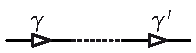
\includegraphics[scale=.8]{positiveNested}} & \raisebox{.3cm}{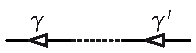
\includegraphics[scale=.8]{negativeNested}} & 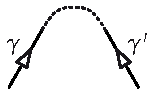
\includegraphics[scale=.8]{negativeDisjoint} & 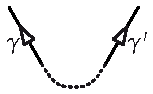
\includegraphics[scale=.8]{positiveDisjoint} \\[.2cm]
          $\so[\gamma] \subseteq \so[\gamma']$ & $\so[\gamma] \supseteq \so[\gamma']$ & $\so[\gamma] \negDisjoint \so[\gamma']$ & $\so[\gamma] \posDisjoint \so[\gamma']$
        \end{tabular}
      }
      \caption{The relative position of two arcs~$\gamma$ and~$\gamma'$ in a signed spine~$\spine$ determines the compatibility relation between their source label sets~$\so[\gamma]$ and~$\so[\gamma]$.}
      \label{fig:sourceSetsCompatible}
    \end{figure}
  \end{itemize}

  \para{Injective}
  To see the injectivity of~$\spineToNested$, we prove that we can reconstruct a spine~$\spine$ from the source sets of its arcs.
  First the the nodes of~$\spine$ are the equivalence classes under the relation~$v \equiv w$ if there is no arc~$\gamma$ of~$\spine$ such that~$|\{v,w\} \cap \so[\gamma]| = 1$.
  Second, the leaves of~$\spine$ correspond to the source sets containing either only one or all but one node of~$\spine$. 
  We can then delete one leaf~$\ell$ of~$\spine$, and reconstruct by induction the tree~$\spine \ssm \{\ell\}$. 
  Finally the only possible node of~$\spine \ssm \{\ell\}$ to which the leaf~$\ell$ can be glued is the unique node which is in the intersection of all source sets~$\chunk$ of~$\spine \ssm \{\ell\}$ such that~$\chunk \cup \ell$ is a source set of~$\spine$, but not in the union of all source sets~$\chunk$ of~$\spine \ssm \{\ell\}$ such that~$\chunk \cup \ell$ is not a source set of~$\spine$.

  \para{Surjective}
  To see the surjectivity of~$\spineToNested$, we prove that for any chunk nested set~$\nested$ on~$\decoratedGraph$,
\begin{enumerate}[(a)]
\item there exists a spine~$\spine$ on~$\decoratedGraph$ such that~$\spineToNested(\spine) = \nested$, and
\item for any chunk~$\chunk$ of~$\decoratedGraph$ compatible with all chunks of~$\nested$, there exists a node~$X$ of~$\spine$ such that the partition~$X = (X \cap \chunk) \sqcup (X \ssm \chunk)$ is splittable (see \cref{def:splittable}).
\end{enumerate}
  These properties are proved by induction on the size of~$\nested$.  
  To initialize, observe that the rank~$0$ spine (with a single node~$\vertexSet$) is sent to the empty chunk nested set for which Property~(b) above holds by \cref{def:chunk}.

  Assume now that these properties hold for a given chunk nested set~$\nested$ and consider a bigger chunk nested set~$\nested' \eqdef \nested \cup \{\chunk\}$.
  Let~$\spine$ be the spine such that~$\spineToNested(\spine) = \nested$ and let~$X$ be a node of~$\spine$ such that the partition~$X = (X \cap \chunk) \sqcup (X \ssm \chunk)$ is splittable.
  Let~$\spine'$ denote the spine obtained by the splitting of~$(X \cap \chunk) \sqcup (X \ssm \chunk)$ in~$\spine$.
  We claim that $\spine$ satisfies Properties (a) and (b) above.
  
  Consider first an incoming arc~$\alpha$ of~$X$ in~$\spine$.
  Since~$\chunk$ is compatible with~$\so[\alpha]$, and both~$X \cap \chunk$ and~$X \ssm \chunk$ are non-empty, we obtain that~$\so[\alpha] \subseteq \chunk$ or~$\so[\alpha] \negDisjoint \chunk$.
  Moreover, by \cref{def:nodeSplitting}, the arc~$\alpha$ is connected to the node~$X \cap \chunk$ of~$\spine'$ if~$\so[\alpha] \subseteq \chunk$, and to the node~$X \ssm \chunk$ of~$\spine'$ if~$\so[\alpha] \negDisjoint \chunk$.
  Similarly, for any outgoing arc~$\beta$ of~$X$ in~$\spine$, we have~$\so[\beta] \supseteq \chunk$ or~$\so[\alpha] \posDisjoint \chunk$, and the arc~$\beta$ is connected to the node~$X \ssm \chunk$ of~$\spine'$ if~$\so[\beta] \supseteq \chunk$, and to the node~$X \cap \chunk$ of~$\spine'$ if~$\so[\beta] \posDisjoint \chunk$.
  In particular, we have~$\so[\alpha] \subseteq \chunk$ for each incoming arc~$\alpha$ of~$X \cap \chunk$ in~$\spine'$, and~$\ta[\beta] \subseteq \chunk$ for each outgoing arc~$\beta$ of~$X \cap \chunk$ in~$\spine'$ (since~$\so[\beta] \posDisjoint \chunk$ implies $\so[\beta] \cup \chunk = \vertexSet$ hence $\ta[\beta] = \vertexSet \ssm \so[\beta] \subseteq \chunk$).
  We thus obtain that~$\so[\gamma] \subseteq \chunk$, and similarly that~$\ta[\gamma] \subseteq \vertexSet \ssm \chunk$, from which we conclude that $\so[\gamma] = \chunk$.
  Since~$\spine'$ is obtained by splitting a node of~$\spine$ into an arc~$\gamma$, we have~$\spineToNested(\spine') = \spineToNested(\spine) \cup \{\so[\gamma]\} = N \cup \{\chunk\} = N '$.

  Consider now another chunk~$\chunk'$ of~$\decoratedGraph$ compatible with all chunks of~$N'$.
  Since~$\chunk'$ is compatible with~$N \subseteq N'$, there is a node~$X'$ of~$\spine$ such that the partition~$X' = (X' \cap \chunk') \sqcup (X' \ssm \chunk')$ is splittable.
  If~$X \ne X'$, then~$X'$ is still a node of~$\spine'$ so that there is nothing to prove.
  If~$X = X'$, then the node~$X \cap \chunk$ of~$\spine'$ suits if~$\chunk \supseteq \chunk'$ or~$\chunk \negDisjoint \chunk'$, while the node~$X \ssm \chunk$ of~$\spine'$  suits if~$\chunk \subseteq \chunk'$ or~$\chunk \posDisjoint \chunk'$.
  \vincent{Check that, maybe add a sentence...}

  \para{Order-preserving}
  Finally, $\spineToNested$ is clearly order preserving as contracting one arc of a spine~$\spine$ removes the corresponding chunk of the chunk nested set~$\spineToNested(\spine)$.
\end{proof}

\begin{remark}
  \label{rem:nestedToSpine}
  From the proof of \cref{prop:spineToNested}, we can give a direct description of the inverse map~$\nestedToSpine$ of the map~$\spineToNested$.
  Namely, consider a chunk nested set~$N$ and two chunks~$\chunk, \chunk'$ of~$N$, and let~$\gamma, \gamma'$ denote the arcs of~$\spine \eqdef \nestedToSpine(N)$ such that~$\so[\gamma] = \chunk$ and~$\so[\gamma'] = \chunk'$.
  Then
  \begin{enumerate}[(i)]
    \item the target of~$\gamma$ and the source of~$\gamma'$ coincide iff~$\chunk \subseteq \chunk'$ and~$\nexists \, \chunk'' \in \nested$ with~$\chunk \subseteq \chunk'' \subseteq \chunk'$ or~$\chunk \negDisjoint \chunk'' \posDisjoint \chunk'$,
    \item the targets of~$\gamma$ and~$\gamma'$ coincide iff~$\chunk \negDisjoint \chunk'$ and~$\nexists \, \chunk'' \in \nested$ with~$\chunk \subseteq \chunk'' \negDisjoint \chunk'$ or~${\chunk \negDisjoint \chunk'' \supseteq \chunk'}$,
\item the sources of~$\gamma$ and~$\gamma'$ coincide iff~$\chunk \posDisjoint \chunk'$ and~$\nexists \, \chunk'' \in \nested$ with~$\chunk \posDisjoint \chunk'' \subseteq \chunk'$ or~${\chunk \supseteq \chunk'' \posDisjoint \chunk'}$.
\end{enumerate}
This gives a description of the nodes of the spine~$\nestedToSpine(\nested)$ in terms of equivalence classes of chunks of~$\nested$ (by the relations above). It also gives a direct definition of the directed graph underlying~$\nestedToSpine(\nested)$ as a quotient of a collection of disjoint arcs labeled by~$\nested$ by identification of some of their endpoints. Finally, each node of~$\nestedToSpine(\nested)$ with incoming arcs~$A$ and outgoing arcs~$\chunk$ is given by
\[
\bigg( \bigcap_{\beta \in \chunk} \so[\beta] \bigg) \ssm \bigg( \bigcup_{\alpha \in A} \so[\alpha] \bigg) = \vertexSet \ssm \bigg( \bigcup_{\alpha \in A} \so[\alpha] \cup \bigcup_{\beta \in \chunk} \ta[\beta] \bigg).
\]
\end{remark}

%%%%%%%%%%%%%%%%%%%%%%%%%%%%%%%%%%%%%%%

\subsection{Flips}
\label{subsec:flips}

In this section, we introduce an elementary local operation on spines on~$\decoratedGraph$, that will enable us to show that the chunk nested complex~$\nestedComplex$ is a closed pseudo-manifold.

\begin{definition}
  \label{def:flip}
  Let $\decoratedGraph$ be a decorated block graph and let $\spine$ be a maximal spine on~$\decoratedGraph$.
  Consider two vertices $X = \{x\}$ and $Y = \{y\}$ of $\spine$ related by an arc $\gamma$. 
  Let $\alpha$ be the incoming arc of $X$ such that~$\so[\alpha]$ and~$Y$ are contained in the same connected component of $\Graph \ssm \Down[X]$, and let $\beta$ be the outgoing arc of $Y$ such that~$\ta[\beta]$ and~$X$ are contained in the same connected component of $\Graph \ssm \Up[Y]$.
  We define $\spine'$ to be the spine obtained from $\spine$ by reversing the orientation of~$\gamma$, grafting the arc~$\alpha$ to~$Y$ and the arc~$\beta$ to~$X$.
  We say that $\spine'$ is obtained from $\spine$ by \defn{flipping} the arc~$\gamma$. 
\end{definition}

\begin{figure}[h!]
  \centerline{
  \begin{tikzpicture}[scale=1.6]  
    \node (N0) at (-0.5,-0.5) {\small $x$};
    \node (N1) at (0.5,0.5) {\small $y$};
    %
    \node (o1) at (-1.2,0.6) {\small $\beta_1$};
    \node (od) at (-0.8,0.6) {\small $\dots$};
    \node (oj) at (-0.3,0.6) {\small $\beta_k$};
    %
    \node (oj1) at (0,1.62) {\small $\beta_{k+1}$};
    \node (ojd) at (0.5,1.6) {\small $\dots$};
    \node (ol) at (1,1.6) {\small $\beta_\ell$};
    %
    \node (2) at (1.5,1.6) {\small $\boldsymbol{\beta}$};
    %
    \node (1) at (-1.5,-1.6) {\small $\boldsymbol{\alpha}$};
    %
    \node (i1) at (-1,-1.6) {\small $\alpha_1$};
    \node (id) at (-0.5,-1.6) {\small $\dots$};
    \node (im) at (0,-1.6) {\small $\alpha_i$};
    %
    \node (im1) at (0.3,-0.62) {\small $\alpha_{i+1}$};
    \node (imd) at (0.8,-0.6) {\small $\dots$};
    \node (ik) at (1.2,-0.6) {\small $\alpha_j$};
    %
    \draw[->,thick] (1)--(N0); 
    \draw[->,thick] (N1)--(2); 
    %
    \draw[->] (N0)--(o1); 
    \draw[->] (N0)--(od);
    \draw[->] (N0)--(oj);
    %  
    \draw[->] (N0)--(N1) node[midway, left] {$\gamma$} ; 
    \draw[->] (N1)--(oj1); 
    \draw[->] (N1)--(ojd);
    \draw[->] (N1)--(ol);
    %
    \draw[->] (i1)--(N0);
    \draw[->] (id)--(N0);
    \draw[->] (im)--(N0); 
    %
    \draw[->] (im1)--(N1); 
    \draw[->] (imd)--(N1);
    \draw[->] (ik)--(N1);
  \end{tikzpicture}
  %
  \raisebox{6.5em}{
  \begin{tikzpicture}[scale=1.2]
    \draw[->] (0,0)--(1,0); 
  \end{tikzpicture}}
  %
  \begin{tikzpicture}[scale=1.6]  
    \node (N0) at (-0.5,0.5) {\small $x$};
    \node (N1) at (0.5,-0.5) {\small $y$};
    %  
    \node (o1) at (-1,1.6) {\small $\beta_1$};
    \node (od) at (-0.5,1.6) {\small $\dots$};
    \node (oj) at (0,1.6) {\small $\beta_k$};
    %  
    \node (oj1) at (0.3,0.62) {\small $\beta_{k+1}$};
    \node (ojd) at (0.8,0.6) {\small $\dots$};
    \node (ol) at (1.2,0.6) {\small $\beta_\ell$};
    %
    \node (i1) at (-1.2,-0.6) {\small $\alpha_1$};
    \node (id) at (-0.8,-0.6) {\small $\dots$};
    \node (im) at (-0.3,-0.6) {\small $\alpha_i$};
    %  
    \node (im1) at (0,-1.62) {\small $\alpha_{i+1}$};
    \node (imd) at (0.5,-1.6) {\small $\dots$};
    \node (ik) at (1,-1.6) {\small $\alpha_j$};
    %
    \node (2) at (-1.5,1.6) {\small $\boldsymbol{\beta}$};
    %
    \node (1) at (1.5,-1.6) {\small $\boldsymbol{\alpha}$};
    %
    \draw[->,thick] (1)--(N1); 
    \draw[->,thick] (N0)--(2); 
    %  
    \draw[->] (N0)--(o1); 
    \draw[->] (N0)--(od);
    \draw[->] (N0)--(oj);
    %    
    \draw[->] (N1)--(N0) node[midway, right] {$\gamma$} ; 
    \draw[->] (N1)--(oj1); 
    \draw[->] (N1)--(ojd);
    \draw[->] (N1)--(ol);
    %  
    \draw[->] (i1)--(N0);
    \draw[->] (id)--(N0);
    \draw[->] (im)--(N0); 
    %  
    \draw[->] (im1)--(N1); 
    \draw[->] (imd)--(N1);
    \draw[->] (ik)--(N1);
  \end{tikzpicture}
  }
  \caption{A spine flip.}
  \label{fig:generalFlip}
\end{figure}

The fact that $\spine'$ is indeed a spine is immediate from the definitions. Contracting $\gamma$ in either $\spine$ or $\spine'$, we obtain the same spine $\spine''$. 

\begin{figure}[h!]
  \centerline{
  \begin{tikzpicture}
    \node (1) at (-0.5, 1.5) {$\blue 1$};
    \node (2) at (-0.5, -0.5) {$\blue \updown[2]$};
    \node (3) at (0, -1.5) {$\blue 3$};
    \node (4) at (-1, 2.5) {$\blue 4$};
    \node (5) at (0, 0.5) {$\blue \up[5]$};
    \node (6) at (0.5, 1.5) {$\blue 6$};
    \node (7) at (-1, -1.5) {$\blue \down[7]$};
    \node (8) at (-1.5, -2.5) {$\blue 8$};
    \node (9) at (1, 2.5) {$\blue \up[9]$};
  %
    \draw[->] (8)--(7); 
    \draw[->] (7)--(2); 
    \draw[->] (3)--(2); 
    \draw[->] (2)--(5) node[midway, left] {$\gamma$}; 
    \draw[->] (5)--(1); 
    \draw[->] (1)--(4); 
    \draw[->] (5)--(6); 
    \draw[->] (6)--(9); 
  \end{tikzpicture}
  %
  \raisebox{6.5em}{
  \begin{tikzpicture}[scale=1.2]
    \draw[->] (0,0)--(1,0); 
  \end{tikzpicture}}
  %
  \begin{tikzpicture}
    \node (1) at (0.5, 0.5) {$\blue 1$};
    \node (2) at (-0.5, 0.5) {$\blue \updown[2]$};
    \node (3) at (-1, -0.5) {$\blue 3$};
    \node (4) at (1, 1.5) {$\blue 4$};
    \node (5) at (0, -0.5) {$\blue \up[5]$};
    \node (6) at (-1, 1.5) {$\blue 6$};
    \node (7) at (0.5, -1.5) {$\blue \down[7]$};
    \node (8) at (1, -2.5) {$\blue 8$};
    \node (9) at (-1.5, 2.5) {$\blue \up[9]$};
    %
    \draw[->] (8)--(7); 
    \draw[->] (7)--(5); 
    \draw[->] (3)--(2); 
    \draw[->] (5)--(2) node[midway, right] {$\gamma$};  
    \draw[->] (5)--(1); 
    \draw[->] (1)--(4); 
    \draw[->] (2)--(6); 
    \draw[->] (6)--(9); 
  \end{tikzpicture}
  }
  \caption{Two maximal spines on the block graph of \cref{fig:mapleBlock}, related by a flip.}
  \label{fig:flip}
  \end{figure} 

\begin{lemma} 
  \label{lemma:coveringpair} 
  The spines~$\spine$ and $\spine'$ are the only spines covering $\spine''$ in the spine poset~$\spinePoset$.
\end{lemma}

\begin{proof}
  This follows from \cref{prop:nodeSplitting,prop:contractionSplitting}.
  \vincent{I don't understand why it is so simple compared to the proof in my paper...}
\end{proof}
  
\begin{definition}
  \label{def:flipGraph}
  The \defn{flip graph} is the graph whose vertices are the maximal spines on~$\decoratedGraph$ and whose egdes are the flips between them.
  In other words, it is the facet-ridge graph of the chunk nested complex~$\nestedComplex$.
\end{definition}

\begin{corollary} 
   The chunk nested complex~$\nestedComplex$ is a closed pseudo-manifold. 
\end{corollary}
  
\begin{definition}
  \label{def:increasingFlip}
  Fix a total order~$\prec$ on~$\vertexSet$.
  The flip from~$\spine$ to~$\spine'$ in \cref{def:flip} is \defn{$\prec$-incresing} if~$x \prec y$ and \defn{$\prec$-decreasing} if $x \succ y$.
  The \defn{$\prec$-increasing flip graph} is the directed graph whose vertices are the maximal spines on~$\decoratedGraph$ and whose arcs are the increasing flips between them.
  The \defn{$\prec$-increasing flip poset} is the transitive closure of the $\prec$-increasing flip graph.
\end{definition}

For instance, the flip of \cref{fig:flip} is increasing with respect to the natural order on $V$.

\begin{example}
  \label{exm:flipPosets}
  For instance, the increasing flip poset is (isomorphic to):
  \begin{enumerate}[(i)]
    \item the \defn{weak order} on permutations of~$\vertexSet$ when $\decoratedGraph$ is complete or undecorated.
    \item the \defn{flip poset on maximal tubings} of~$\Graph$ studied in~\cite{BarnardMcConville} when~$\decoratedGraph$ is down decorated (in particular the classical \defn{Tamari lattice}~\cite{Tamari, HuangTamari} when~$\decoratedGraph$ is a down decorated path).
    \item the \defn{acyclic reorientation lattice} of~$\Graph$~\cite{Pilaud-acyclicReorientationLattices} when~$\decoratedGraph$ is fully decorated (in particular the \defn{boolean lattice} when~$\decoratedGraph$ is a fully decorated tree).
    \item the various \defn{permutree lattices} of~\cite{PilaudPons-permutrees} when~$\Graph$ is a path (in particular the various type~$A$ \defn{Cambrian lattices}~\cite{Reading-CambrianLattices} for up-down decorated paths).
  \end{enumerate}
\end{example}

\begin{remark}
  The question of whether or not the increasing flip poset is a lattice is a difficult question. It depends on the decoration $\decoration$. We know that if $\Graph$ is a path, it is always the case \cite{PilaudPons-permutrees}, for $\Graph$ a block graph it is generally not true. See \cite{BarnardMcConville}. \guillaume{Nos calculs?; donner un exemple, un contre-exemple}\vincent{improve this remark.}
\end{remark}

%%%%%%%%%%%%%%%%%%%%%%%%%%%%%%%%%%%%%%%

\subsection{Labeled spines and blossoming spines}
\label{subsec:blossomingSpines}

For later purposes, we now add further information to a spine on~$\decoratedGraph$.
Here, we need to manipulate both the vertices and the cliques of~$\Graph$, thus we consider a maple tree~$\Maple$ corresponding to the block graph~$\Graph$.

\begin{definition}
  \label{def:labeledSpine}
  Let~$\decoratedMaple \eqdef (\Maple, \decoration)$ be a decorated maple tree and~$\decoratedGraph \eqdef (\Graph, \decoration)$ be the decorated block graph obtained by tapping~$\Maple$.
  In a spine~$\spine$ on~$\decoratedGraph$, we label
  \begin{itemize}
    \item each node~$X$ by the connected component~$\labeling(X)$ of~$\Maple \ssm \big( \Up[{\so[X]}] \cup \Down[{\ta[X]}] \big)$ containing~$X$,
%    \item each arc~$\gamma$ by the intersection~$\labeling(\gamma)$ of the connected component of~$\Maple \ssm \Up[{\so[\gamma]}]$ containing~$\ta[\gamma]$ with the connected component of~$\Maple \ssm \Down[{\ta[\gamma]}]$ containing~$\so[\gamma]$.
    \item each arc~$\gamma$ by the connected component~$\labeling(\gamma)$ of~$\Maple \ssm \big( \Up[{\so[\gamma]}] \cup \Down[{\ta[\gamma]}] \big)$ containing the red vertices of~$\Maple$ adjacent to both~$\so[\gamma]$ and~$\ta[\gamma]$. \guillaume{ce ne sont pas tous les sommets de $\Maple$?}
  \end{itemize}
  We say that the spine~$\spine$ with its labeling~$\labeling$ is a \defn{labeled spine}.
\end{definition}

\begin{remark}
  \label{rem:labeledSpine1}
  By definition, the labels of \cref{def:labeledSpine} are some maple subtrees of~$\Maple$.
  Note that a maple subtree of~$\Maple$ is completely determined by its leaves, hence by its red vertices.
  We thus simplify all pictures of labeled spines by writing only the red (letters) vertices of each label.
  For instance, \cref{fig:labeledSpines} illustrates this labeling for the two spines of \cref{fig:spines}.
%
\begin{figure}[h!]
  \centerline{
  \begin{tikzpicture}
    \node[label=west:{\scriptsize \red \textit{abcdefghijk}}] (256) at (0,0) {$\blue \updown[2] \up[5] 6$};
    \node[label=west:{\scriptsize \red \textit{ade}}] (14) at (-1, 2) {$\blue 1 4$};
    \node[label=east:{\scriptsize \red \textit{fgjk}}] (9) at (1, 2) {$\blue \up[9]$};
    \node[label=west:{\scriptsize \red \textit{adefghijk}}] (78) at (-1, -2) {$\blue \down[7] 8$};
    \node[label=east:{\scriptsize \red \textit{bc}}] (3) at (1, -2) {$\blue 3$};
    %
    \draw[->] (256)--(14) node[midway, left] {\scriptsize \red \textit{ade}}; 
    \draw[->] (256)--(9) node[midway, right] {\scriptsize \red \textit{fgjk}}; 
    \draw[->] (78)--(256) node[midway, left] {\scriptsize \red \textit{adefghijk}}; 
    \draw[->] (3)--(256) node[midway, right] {\scriptsize \red \textit{bc}}; 
  \end{tikzpicture}
  %
  \qquad
  %
  \begin{tikzpicture}
    \node[label=west:{\scriptsize \red \textit{ade}}] (1) at (-0.5, 1.5) {$\blue 1$};
    \node[label=west:{\scriptsize \red \textit{abcdefghijk}}] (2) at (-0.5, -0.5) {$\blue \updown[2]$};
    \node[label=east:{\scriptsize \red \textit{bc}}] (3) at (0, -1.5) {$\blue 3$};
    \node[label=west:{\scriptsize \red \textit{ade}}] (4) at (-1, 2.5) {$\blue 4$};
    \node[label=west:{\scriptsize \red \textit{adefghijk}}] (5) at (0, 0.5) {$\blue \up[5]$};
    \node[label=east:{\scriptsize \red \textit{fgjk}}] (6) at (0.5, 1.5) {$\blue 6$};
    \node[label=west:{\scriptsize \red \textit{adefghijk}}] (7) at (-1, -1.5) {$\blue \down[7]$};
    \node[label=west:{\scriptsize \red \textit{adefghjk}}] (8) at (-1.5, -2.5) {$\blue 8$};
    \node[label=east:{\scriptsize \red \textit{jgjk}}] (9) at (1, 2.5) {$\blue \up[9]$};
    %
    \draw[->] (8)--(7) node[midway, left] {\scriptsize \red \textit{adefghjk}}; 
    \draw[->] (7)--(2) node[midway, left] {\scriptsize \red \textit{adefghijk}}; 
    \draw[->] (3)--(2) node[midway, right] {\scriptsize \red \textit{bc}}; 
    \draw[->] (2)--(5) node[midway, left] {\scriptsize \red \textit{adefghijk}}; 
    \draw[->] (5)--(1) node[midway, left] {\scriptsize \red \textit{ade}}; 
    \draw[->] (1)--(4) node[midway, left] {\scriptsize \red \textit{ade}}; 
    \draw[->] (5)--(6) node[midway, right] {\scriptsize \red \textit{fgjk}}; 
    \draw[->] (6)--(9) node[midway, right] {\scriptsize \red \textit{fgjk}}; 
  \end{tikzpicture}
  }
  \caption{The labeled versions of the two spines of \cref{fig:spines}.}
  \label{fig:labeledSpines}
\end{figure} 
\end{remark}

\begin{remark}
  \label{rem:labeledSpine2}
  The labeling~$\labeling$ of \cref{def:labeledSpine} can be described alternatively using \cref{coro:splittablePartitions}.
  For any arc~$\gamma$ in a spine~$\spine$, denote by~$C_\gamma$ the connected component of~$\Maple \ssm \Up[{\so[\gamma]}]$ containing~$\ta[\gamma]$ and by~$C^\gamma$ the connected component of~$\Maple \ssm \Down[{\ta[\gamma]}]$ containing~$\so[\gamma]$.
%  For any arc~$\gamma$ in a spine~$\spine$, denote by~$C_\gamma$ (resp.~$C^\gamma$) the connected component of~$\Maple \ssm \Up[{\so[\gamma]}]$ (resp.~$\Maple \ssm \Down[{\ta[\gamma]}]$) containing~$\ta[\gamma]$ (resp.~$\so[\gamma]$).
  Then 
  \begin{itemize}
    \item $\labeling(X) = \bigcap_\alpha C_\alpha \; \cap \; \bigcap_\beta C^\beta$ where $\alpha$ (resp.~$\beta$) runs over incoming (resp.~outgoing) arcs~of~$X$,
    \item $\labeling(\gamma) = C_\gamma \cap C^\gamma$.
  \end{itemize}     
\end{remark}

\begin{lemma}
  \label{lem:labeledSpine}
%  We have~$\labeling(\alpha) \cap \labeling(\alpha') = \varnothing$ for two incoming arcs~$\alpha, \alpha'$ at the same node~$X$ of~$\spine$.
  We have~$\labeling(\gamma) \cap \labeling(\gamma') = \varnothing$ for any two distinct arcs~$\gamma, \gamma'$ incoming at (resp.~outgoing from) the same node of~$\spine$.
\end{lemma}

\begin{proof}
  Assume for instance that~$\alpha, \alpha'$ are distinct incoming arcs at a node~$X$ of~$\spine$.
  By \cref{def:spine}, the source sets~$\so[\alpha]$ and~$\so[\alpha']$ belong to distinct connected components~$C$ and~$C'$ of~$\Maple \ssm \Down[X]$.
  Moreover, $\labeling(\alpha) \subseteq C$ since~$X \subseteq \ta[\alpha]$ and similarly~$\labeling(\alpha') \subseteq C'$.
  Hence~$\labeling(\alpha) \cap \labeling(\alpha') = \varnothing$.
\end{proof}

We now add a little more to a labeled spine.
This is not strictly needed for the purposes of the next section, but it enlightens the picture and will simplify some proofs in later sections.
\vincent{also needed for the operad part...}

\begin{definition}
  \label{def:blossomingTree}
  A \defn{directed blossoming tree} is a directed tree~$\spine$ with some additional 
  \begin{itemize}
    \item \defn{incoming blossoms} (arcs joining an empty node to a normal node) and 
    \item \defn{outgoing blossoms} (arcs joining a normal node to an empty node).
  \end{itemize}
  A \defn{cut} of a directed blossoming tree~$\spine$ is a set~$\Gamma$ of nodes, arcs and blossoms of~$\spine$ such that any directed path joining the source of an incoming blossom of~$\spine$ to the target of an outgoing blossom of~$\spine$ contains precisely one element of~$\Gamma$.
  When the nodes of~$\spine$ are sets, the \defn{source set}~$\so[\Gamma]$ (resp.~\defn{target set}~$\ta[\Gamma]$) of~$\Gamma$ is the union of the nodes of all connected components of~$\spine \ssm \Gamma$ which contain the source (resp.~target) of an incoming blossom.
  For instance, the set of incoming (resp.~outgoing) blossoms is a cut of~$\spine$ whose source (resp.~target) set is empty and whose target (resp.~source) set is the union of the nodes of~$\spine$.
\end{definition}

\begin{definition}
  \label{def:blossomingSpine}
  Let~$\decoratedMaple \eqdef (\Maple, \decoration)$ be a decorated maple tree, let~$\decoratedGraph \eqdef (\Graph, \decoration)$ be the decorated block graph obtained by tapping~$\Maple$, and let~$\spine$ be a spine on~$\decoratedGraph$.
  The \defn{blossoming spine}~$\spine\blossom$ is the labeled blossoming tree obtained from the labeled spine~$\spine$ by a adding at each node~$X$ of~$\spine$ an incoming (resp.~outgoing) blossom labeled by~$C$ for each connected component~$C$ of~$\Maple \ssm \Down[\vertexSet]$ (resp.~of~$\Maple \ssm \Up[\vertexSet]$) adjacent to~$X$ such that there is no incoming arc~$\alpha$ (resp.~outgoing arc~$\beta$) of~$X$ with~$\so[\alpha]$ (resp.~$\ta[\beta]$) contained in~$C$.
\end{definition}

\begin{remark}
  As in \cref{rem:labeledSpine1}, it is sufficient in the pictures to write only the red vertices of each label.
  For instance, \cref{fig:blossomingSpines} illustrates the blossoming spines of the two spines of \cref{fig:spines}.
%
\begin{figure}[h!]
  \centerline{
  \begin{tikzpicture}
    \node[label=west:{\scriptsize \red \textit{abcdefghijk}}] (256) at (0,0) {$\blue \updown[2] \up[5] 6$};
    \node[label=west:{\scriptsize \red \textit{ade}}] (14) at (-1, 2) {$\blue 1 4$};
    \node[label=east:{\scriptsize \red \textit{fgjk}}] (9) at (1, 2) {$\blue \up[9]$};
    \node[label=west:{\scriptsize \red \textit{adefghijk}}] (78) at (-1, -2) {$\blue \down[7] 8$};
    \node[label=east:{\scriptsize \red \textit{bc}}] (3) at (1, -2) {$\blue 3$};
    \node (i) at (-0.5, -3) {};
    \node (adefghjk) at (-1.5, -3) {};
    \node (bc) at (1.5, -3) {};
    \node (bc') at (.8, 0.7) {};
    \node (hi') at (0, 1) {};
    \node (ade') at (-1.5, 3) {};
    \node (fgj') at (0.5, 3) {};
    \node (k') at (1.5, 3) {};
    %
    \draw[->] (256)--(14) node[midway, left] {\scriptsize \red \textit{ade}}; 
    \draw[->] (256)--(9) node[midway, right] {\scriptsize \red \textit{fgjk}}; 
    \draw[->] (78)--(256) node[midway, left] {\scriptsize \red \textit{adefghijk}}; 
    \draw[->] (3)--(256) node[midway, right] {\scriptsize \red \textit{bc}}; 
    \draw[->] (i)--(78) node[midway, right] {\scriptsize \red \textit{i}}; 
    \draw[->] (adefghjk)--(78) node[midway, left] {\scriptsize \red \textit{adefghjk}};
    \draw[->] (bc)--(3) node[midway, right] {\scriptsize \red \textit{bc}}; 
    \draw[->] (9)--(k') node[midway, right] {\scriptsize \red \textit{k}}; 
    \draw[->] (9)--(fgj') node[midway, left] {\scriptsize \red \textit{fgj}};
    \draw[->] (14)--(ade') node[midway, left] {\scriptsize \red \textit{ade}};
    \draw[->] (256)--(bc') node[midway, right] {\scriptsize \red \textit{bc}};
    \draw[->] (256)--(hi') node[midway, left] {\scriptsize \red \textit{hi}};
  \end{tikzpicture}
  %
  \qquad
  %
  \begin{tikzpicture}
    \node[label=west:{\scriptsize \red \textit{ade}}] (1) at (-0.5, 1.5) {$\blue 1$};
    \node[label=west:{\scriptsize \red \textit{abcdefghijk}}] (2) at (-0.5, -0.5) {$\blue \updown[2]$};
    \node[label=east:{\scriptsize \red \textit{bc}}] (3) at (0, -1.5) {$\blue 3$};
    \node[label=west:{\scriptsize \red \textit{ade}}] (4) at (-1, 2.5) {$\blue 4$};
    \node[label=west:{\scriptsize \red \textit{adefghijk}}] (5) at (0, 0.5) {$\blue \up[5]$};
    \node[label=east:{\scriptsize \red \textit{fgjk}}] (6) at (0.5, 1.5) {$\blue 6$};
    \node[label=west:{\scriptsize \red \textit{adefghijk}}] (7) at (-1, -1.5) {$\blue \down[7]$};
    \node[label=west:{\scriptsize \red \textit{adefghjk}}] (8) at (-1.5, -2.5) {$\blue 8$};
    \node[label=east:{\scriptsize \red \textit{jgjk}}] (9) at (1, 2.5) {$\blue \up[9]$};
    \node (adefghjk) at (-2, -3.5) {};
    \node (i) at (-0.5, -2.5) {};
    \node (bc) at (0.5, -2.5) {};
    \node (bc') at (.5, -.2) {};
    \node (hi') at (1, .8) {};
    \node (ade') at (-1.5, 3.5) {};
    \node (fgj') at (0.5, 3.5) {};
    \node (k') at (1.5, 3.5) {};
    %
    \draw[->] (8)--(7) node[midway, left] {\scriptsize \red \textit{adefghjk}}; 
    \draw[->] (7)--(2) node[midway, left] {\scriptsize \red \textit{adefghijk}}; 
    \draw[->] (3)--(2) node[midway, right] {\scriptsize \red \textit{bc}}; 
    \draw[->] (2)--(5) node[midway, left] {\scriptsize \red \textit{adefghijk}}; 
    \draw[->] (5)--(1) node[midway, left] {\scriptsize \red \textit{ade}}; 
    \draw[->] (1)--(4) node[midway, left] {\scriptsize \red \textit{ade}}; 
    \draw[->] (5)--(6) node[midway, right] {\scriptsize \red \textit{fgjk}}; 
    \draw[->] (6)--(9) node[midway, right] {\scriptsize \red \textit{fgjk}}; 
    \draw[->] (4)--(ade') node[midway, left] {\scriptsize \red \textit{ade}}; 
    \draw[->] (9)--(fgj') node[midway, left] {\scriptsize \red \textit{fgj}}; 
    \draw[->] (9)--(k') node[midway, right] {\scriptsize \red \textit{k}}; 
    \draw[->] (adefghjk)--(8) node[midway, left] {\scriptsize \red \textit{adefghjk}}; 
    \draw[->] (i)--(7) node[midway, right] {\scriptsize \red \textit{i}}; 
    \draw[->] (bc)--(3) node[midway, right] {\scriptsize \red \textit{bc}};
    \draw[->] (2)--(bc') node[midway, right] {\scriptsize \red \textit{bc}};
    \draw[->] (5)--(hi') node[midway, right] {\scriptsize \red \textit{hi}};
  \end{tikzpicture}
  }
  \caption{The blossoming versions of the two spines of \cref{fig:spines}.}
  \label{fig:blossomingSpines}
\end{figure}
\end{remark}

\begin{proposition}
  \label{prop:blossomingSpine}
  Let~$\decoratedMaple \eqdef (\Maple, \decoration)$ be a decorated maple tree, let~$\decoratedGraph \eqdef (\Graph, \decoration)$ be the decorated block graph obtained by tapping~$\Maple$, and let~$\spine$ be a spine on~$\decoratedGraph$.
  For any cut~$\Gamma$ of~$\spine\blossom$, the labels of the nodes, arcs and blossoms of~$\Gamma$ are precisely the connected components of~$\Maple \ssm \big( \Up[{\so[\Gamma]}] \cup \Down[{\ta[\Gamma]}] \big)$.
\end{proposition}

\begin{proof}
  We prove the result by sweeping the blossoming spine~$\spine\blossom$.

  The base case is the cut~$\Gamma_\circ$ of~$\spine\blossom$ consisting of all its incoming blossoms, which are labeled by the connected components of~$\Maple \ssm \Down[\vertexSet]$.
  Indeed, the label of any incoming blossom is a connected component of~$\Maple \ssm \Down[\vertexSet]$ by definition.
  Conversely, for any connected component~$C$ of~$\Maple \ssm \Down[\vertexSet]$, the set of nodes of~$\spine$ adjacent to~$C$ forms a chain in~$\spine$ by \cref{def:spine}, and~$C$ appears as an incoming blossom of the minimal node of~$\spine$ in this chain.
  
%  Consider now a node~$X$ of~$\spine\blossom$, and let~$A$ denote its set of incoming arcs and blossoms.
  Consider now two cuts~$\Gamma$ and~$\Gamma'$ of~$\spine\blossom$ such that~$\Gamma \ssm A = \Gamma' \ssm \{X\}$ where~$A$ is the set of incoming arcs and blossoms of a node~$X$ of~$\spine\blossom$.
  Note that the sets~$\labeling(\alpha)$ for~$\alpha \in A$ are precisely the connected components of~$\Maple \ssm \big( \Up[{\so[\Gamma]}] \cup \Down[{\ta[\Gamma]}] \big)$ adjacent to~$X$, and that $\labeling(X)$ is the connected component of~$\Maple \ssm \big( \Up[{\so[\Gamma']}] \cup \Down[{\ta[\Gamma']}] \big)$ containing~$X$.
  We conclude that if the result holds for~$\Gamma$, then it also holds for~$\Gamma'$.
  The argument is symmetric for two cuts~$\Gamma$ and~$\Gamma'$ of~$\spine\blossom$ such that~$\Gamma \ssm \{X\} = \Gamma' \ssm B$ where~$B$ is the set of outgoing arcs and blossoms of a node~$X$ of~$\spine\blossom$.
  The result thus follows since any cut of~$\spine\blossom$ can be obtained from the cut~$\Gamma_\circ$ by a sequence of such moves.
\end{proof}
%
%\begin{figure}[h!]
%  \begin{tikzpicture}
%    \node (0) at (0, 0) {$\updown[2] \up[5] 6$};
%    \node (1) at (-3, 1) {$ade$};
%    \node (2) at (-1, 1) {$hi$};
%    \node (3) at (1, 1) {$fgjk$};
%    \node (4) at (3, 1) {$bc$};
%    \node (5) at (3, 3) {$bc$};
%    \node (6) at (1.5, 3) {$k$};
%    \node (7) at (0.5, 3) {$fgj$};
%    \node (8) at (-1, 3) {$hi$};
%    \node (9) at (-3, 3) {$ade$};
%    \node (10) at (1, 2) {$\up[9]$};
%    \node (11) at (-3, 2) {$14$};
%    \node (12) at (-1, -1) {$adefghijk$};
%    \node (13) at (1, -1) {$bc$};
%    \node (14) at (-1, -2) {$\down[7] 8$};
%    \node (15) at (1, -2) {$3$};
%    \node (16) at (-2, -3) {$adefghjk$};
%    \node (17) at (0, -3) {$i$};
%    \node (18) at (1, -3) {$bc$};
%    \draw[->] (18)--(15);
%    \draw[->] (17)--(14);
%    \draw[->] (16)--(14);
%    \draw[->] (15)--(13);
%    \draw[->] (14)--(12);
%    \draw[->] (13)--(0);
%    \draw[->] (12)--(0);
%    \draw[->] (0)--(1);
%    \draw[->] (0)--(2);
%    \draw[->] (0)--(3);
%    \draw[->] (0)--(4);
%    \draw[->] (1)--(11);
%    \draw[->] (2)--(8);
%    \draw[->] (3)--(10);
%    \draw[->] (4)--(5);
%    \draw[->] (11)--(9);
%    \draw[->] (10)--(7);
%    \draw[->] (10)--(6);
%    \draw[dotted] (-5,-3)--(16)--(17)--(18)--(5,-3);
%    \draw[dashed] (-5,-2)--(14)--(15)--(5,-2);
%    \draw[dotted] (-5,-1)--(12)--(13)--(5,-1);
%    \draw[dashed] (-5,0)--(0)--(5,0);
%    \draw[dotted] (-5,1)--(1)--(2)--(3)--(4)--(5,1);
%    \draw[dashed] (-5,2)--(11)--(10)--(5,2);
%    \draw[dotted] (-5,3)--(9)--(8)--(7)--(6)--(5)--(5,3);
%    \node (20) at (5.5, -3) {$\down[2] \down[7]$};
%    \node (21) at (5.5, -2) {$\down[2]$};
%    \node (22) at (5.5, -1) {$\down[2]$};
%    \node (23) at (5.5, 0) {};
%    \node (24) at (5.5, 1) {$\up[2] \up[5]$};
%    \node (25) at (5.5, 2) {$\up[2] \up[5]$};
%    \node (26) at (5.5, 3) {$\up[2] \up[5] \up[9]$};
%  \end{tikzpicture}
%  \caption{A blossoming spine on the maple tree of \cref{fig:mapleBlock}, reconstructed from $\pi = 3 \down[7] 8 | \updown[2] \up[5] 6 | 149$.}
%  \label{fig:blossomingSpine}
%\end{figure}

%%%%%%%%%%%%%%%%%%%%%%%%%%%%%%%%%%%%%%%

\subsection{Refinement and surjection maps}
\label{subsec:surjectionMaps}

We now consider a natural refinement order on decorated block graphs and define natural surjections between the spines of refining decorated block graphs.

\begin{definition}
  \label{def:refinementDecoratedGraphs}
  For two decorations~$\decoration$ and~$\decoration'$ on a set~$\vertexSet$, we say that~$\decoration$ \defn{refines}~$\decoration'$ (and that $\decoration'$ \defn{coarsens} $\decoration$) if~$\Down[\vertexSet] \subseteq \Down[\vertexSet][\decoration']$ and $\Up[\vertexSet] \subseteq \Up[\vertexSet][\decoration']$.
  For two decorated block graphs~$\decoratedGraph \eqdef (\Graph, \decoration)$ and~$\decoratedGraph' \eqdef (\Graph', \decoration')$, we say that~$\decoratedGraph$ \defn{refines}~$\decoratedGraph'$ (and that $\decoratedGraph'$ \defn{coarsens} $\decoratedGraph$) if~$\Graph = \Graph'$ and $\decoration$ refines~$\decoration'$.
\end{definition}

\begin{figure}
  \centerline{
  \begin{tikzpicture}[scale=.7]  
    \node (1) at (-4, -19) {$\blue 1$};
    \node (2) at (0, -19) {$\blue \down[2]$};
    \node (3) at (2, -19) {$\blue 3$};
    \node (4) at (-4, -21) {$\blue 4$};
    \node (5) at (-2, -21) {$\blue \up[5]$};
    \node (6) at (2, -21) {$\blue 6$};
    \node (7) at (-4, -23) {$\blue 7$};
    \node (8) at (0, -23) {$\blue 8$};
    \node (9) at (2, -23) {$\blue 9$};
    %
    \node (a) at (-5, -19) {$\red a$};
    \node (b) at (1, -19) {$\red b$};
    \node (c) at (3, -19) {$\red c$};
    \node (d) at (-3, -20) {$\red d$};
    \node (e) at (-5, -21) {$\red e$};
    \node (f) at (0, -21) {$\red f$};
    \node (g) at (3, -21) {$\red g$};
    \node (h) at (-3, -22) {$\red h$};
    \node (i) at (-5, -23) {$\red i$};
    \node (j) at (1, -23) {$\red j$};
    \node (k) at (3, -23) {$\red k$};
    %
    \draw[-] (a)--(1)--(d)--(4)--(e); 
    \draw[-] (d)--(5)--(h)--(7)--(i); 
    \draw[-] (5)--(f)--(6)--(g); 
    \draw[-] (c)--(3)--(b)--(2)--(f)--(8)--(j)--(9)--(k); 
  \end{tikzpicture}
  %
  \qquad
  %
  \begin{tikzpicture}[scale=.7]  
    \node (1) at (-4, -19) {$\blue 1$};
    \node (2) at (0, -19) {$\blue \updown[2]$};
    \node (3) at (2, -19) {$\blue 3$};
    \node (4) at (-4, -21) {$\blue 4$};
    \node (5) at (-2, -21) {$\blue \updown[5]$};
    \node (6) at (2, -21) {$\blue \up[6]$};
    \node (7) at (-4, -23) {$\blue \down[7]$};
    \node (8) at (0, -23) {$\blue \updown[8]$};
    \node (9) at (2, -23) {$\blue 9$};
    %
    \node (a) at (-5, -19) {$\red a$};
    \node (b) at (1, -19) {$\red b$};
    \node (c) at (3, -19) {$\red c$};
    \node (d) at (-3, -20) {$\red d$};
    \node (e) at (-5, -21) {$\red e$};
    \node (f) at (0, -21) {$\red f$};
    \node (g) at (3, -21) {$\red g$};
    \node (h) at (-3, -22) {$\red h$};
    \node (i) at (-5, -23) {$\red i$};
    \node (j) at (1, -23) {$\red j$};
    \node (k) at (3, -23) {$\red k$};
    %
    \draw[-] (a)--(1)--(d)--(4)--(e); 
    \draw[-] (d)--(5)--(h)--(7)--(i); 
    \draw[-] (5)--(f)--(6)--(g); 
    \draw[-] (c)--(3)--(b)--(2)--(f)--(8)--(j)--(9)--(k); 
  \end{tikzpicture}
  }
  \caption{The left decorated maple tree~$\decoratedMaple$ refines the right decorated maple tree~$\decoratedMaple'$.}
  \label{fig:refinementDecoratedGraphs}
\end{figure} 

\begin{figure}[h!]
  \centerline{    
  \begin{tikzpicture}
    \node[label=west:{\scriptsize \red \textit{adefghijk}}] (79) at (0,1) {$\blue 7 9$};
    \node[label=west:{\scriptsize \red \textit{abcdefghijk}}] (248) at (0,2) {$\blue \down[2] 4 8$};
    \node[label=west:{\scriptsize \red \textit{abcdefghijk}}] (35) at (0,3) {$\blue 3 \up[5]$};
    \node[label=west:{\scriptsize \red \textit{ade}}] (1) at (-.5,4) {$\blue 1$};
    \node[label=east:{\scriptsize \red \textit{bcfgjk}}] (6) at (.5,4) {$\blue 6$};
    %
    \draw[->] (79)--(248) node[midway, left] {\scriptsize \red \textit{adefghijk}};
    \draw[->] (248)--(35) node[midway, left] {\scriptsize \red \textit{abcdefghijk}};
    \draw[->] (35)--(1) node[midway, left] {\scriptsize \red \textit{ade}};
    \draw[->] (35)--(6) node[midway, right] {\scriptsize \red \textit{bcfgjk}};
  \end{tikzpicture}
  %
  \qquad
  %
  \begin{tikzpicture}
    \node[label=east:{\scriptsize \red \textit{hi}}] (7) at (1,1) {$\blue \down[7]$};
    \node[label=east:{\scriptsize \red \textit{jk}}] (9) at (3,1) {$\blue 9$};
    \node[label=west:{\scriptsize \red \textit{ade}}] (4) at (0,2) {$\blue 4$};
    \node[label=east:{\scriptsize \red \textit{bcfgjk}}] (28) at (3,2) {$\blue \updown[2] \updown[8]$};
    \node[label=west:{\scriptsize \red \textit{adefghi}}] (5) at (1,3) {$\blue \updown[5]$};
    \node[label=east:{\scriptsize \red \textit{bc}}] (3) at (4,3) {$\blue 3$};
    \node[label=west:{\scriptsize \red \textit{ade}}] (1) at (0,4) {$\blue 1$};
    \node[label=east:{\scriptsize \red \textit{fg}}] (6) at (2,4) {$\blue \up[6]$};
    \node[label=west:{\scriptsize \red \textit{ade}}] (e1) at (0,1) {$\blue \varnothing$};
    \node[label=west:{\scriptsize \red \textit{fg}}] (e2) at (2,1) {$\blue \varnothing$};
    \node[label=east:{\scriptsize \red \textit{hi}}] (e3) at (1,2) {$\blue \varnothing$};
    \node[label=west:{\scriptsize \red \textit{jk}}] (e4) at (3,3) {$\blue \varnothing$};
    \node[label=west:{\scriptsize \red \textit{jk}}] (e5) at (3,4) {$\blue \varnothing$};
    \node[label=east:{\scriptsize \red \textit{bc}}] (e6) at (4,4) {$\blue \varnothing$};
    %
    \draw[->] (e1)--(4) node[midway, left] {\scriptsize \red \textit{ade}};
    \draw[->] (7)--(e3) node[midway, right] {\scriptsize \red \textit{hi}};
    \draw[->] (e2)--(28) node[midway, left] {\scriptsize \red \textit{fg}};
    \draw[->] (9)--(28) node[midway, right] {\scriptsize \red \textit{jk}};
    \draw[->] (4)--(5) node[midway, left] {\scriptsize \red \textit{ade}};
    \draw[->] (e3)--(5) node[midway, right] {\scriptsize \red \textit{hi}};
    \draw[->] (28)--(5) node[midway, right] {\scriptsize \red \textit{fg}};
    \draw[->] (28)--(e4) node[midway, left] {\scriptsize \red \textit{jk}};
    \draw[->] (28)--(3) node[midway, right] {\scriptsize \red \textit{bc}};
    \draw[->] (5)--(1) node[midway, left] {\scriptsize \red \textit{ade}};
    \draw[->] (5)--(6) node[midway, right] {\scriptsize \red \textit{fg}};
    \draw[->] (e4)--(e5) node[midway, left] {\scriptsize \red \textit{jk}};
    \draw[->] (3)--(e6) node[midway, right] {\scriptsize \red \textit{bc}};
  \end{tikzpicture}    
  %
  \qquad
  %
  \begin{tikzpicture}
    \node[label=east:{\scriptsize \red \textit{hi}}] (7) at (1,1) {$\blue \down[7]$};
    \node[label=east:{\scriptsize \red \textit{jk}}] (9) at (2.5,1) {$\blue 9$};
    \node[label=west:{\scriptsize \red \textit{ade}}] (4) at (0,2) {$\blue 4$};
    \node[label=east:{\scriptsize \red \textit{bcfgjk}}] (28) at (2.5,2) {$\blue \updown[2] \updown[8]$};
    \node[label=west:{\scriptsize \red \textit{adefghi}}] (5) at (1,3) {$\blue \updown[5]$};
    \node[label=east:{\scriptsize \red \textit{bc}}] (3) at (2.5,3) {$\blue 3$};
    \node[label=west:{\scriptsize \red \textit{ade}}] (1) at (0,4) {$\blue 1$};
    \node[label=east:{\scriptsize \red \textit{fg}}] (6) at (2,4) {$\blue \up[6]$};
    %
    \draw[->] (7)--(5) node[midway, right] {\scriptsize \red \textit{hi}};
    \draw[->] (9)--(28) node[midway, right] {\scriptsize \red \textit{jk}};
    \draw[->] (4)--(5) node[midway, left] {\scriptsize \red \textit{ade}};
    \draw[->] (28)--(5) node[midway, right] {\scriptsize \red \textit{fg}};
    \draw[->] (28)--(3) node[midway, right] {\scriptsize \red \textit{bc}};
    \draw[->] (5)--(1) node[midway, left] {\scriptsize \red \textit{ade}};
    \draw[->] (5)--(6) node[midway, right] {\scriptsize \red \textit{fg}};
  \end{tikzpicture}
  }
  \caption{A spine~$\spine$ on~$\decoratedMaple$ (left) and the spine~$\spine' = \surjectionSpines(\spine)$ on~$\decoratedMaple'$ (right) obtained by contracting the empty node in the directed tree~$\almostSpine$ (middle) defined in \cref{def:refinementSpines}.}
  \label{fig:refinementSpines}
\end{figure} 

\begin{figure}[h!]
  \centerline{    
  \begin{tikzpicture}
    \node[label=west:{\scriptsize \red \textit{adefghijk}}] (79) at (0,1) {$\blue 7 9$};
    \node[label=west:{\scriptsize \red \textit{abcdefghijk}}] (248) at (0,2) {$\blue \down[2] 4 8$};
    \node[label=west:{\scriptsize \red \textit{abcdefghijk}}] (35) at (0,3) {$\blue 3 \up[5]$};
    \node[label=west:{\scriptsize \red \textit{ade}}] (1) at (-1,4) {$\blue 1$};
    \node[label=east:{\scriptsize \red \textit{bcfgjk}}] (6) at (1,4) {$\blue 6$};
    \node (adefghijk) at (0,0) {};
    \node (bc) at (.8,1.2) {};
    \node (ade') at (-1,5) {};
    \node (hi') at (0,4) {};
    \node (bcfgjk') at (1,5) {};
    %
    \draw[->] (adefghijk)--(79) node[midway, left] {\scriptsize \red \textit{adefghijk}};
    \draw[->] (79)--(248) node[midway, left] {\scriptsize \red \textit{adefghijk}};
    \draw[->] (bc)--(248) node[midway, right] {\scriptsize \red \textit{bc}};
    \draw[->] (248)--(35) node[midway, left] {\scriptsize \red \textit{abcdefghijk}};
    \draw[->] (35)--(1) node[midway, left] {\scriptsize \red \textit{ade}};
    \draw[->] (35)--(6) node[midway, right] {\scriptsize \red \textit{bcfgjk}};
    \draw[->] (35)--(hi') node[midway, right] {\scriptsize \red \textit{hi}};
    \draw[->] (1)--(ade') node[midway, left] {\scriptsize \red \textit{ade}};
    \draw[->] (6)--(bcfgjk') node[midway, right] {\scriptsize \red \textit{bcfgjk}};
  \end{tikzpicture}
  %
  \quad
  %
  \begin{tikzpicture}
    \node[label=east:{\scriptsize \red \textit{hi}}] (7) at (1.5,1) {$\blue \down[7]$};
    \node[label=east:{\scriptsize \red \textit{jk}}] (9) at (4,1) {$\blue 9$};
    \node[label=west:{\scriptsize \red \textit{ade}}] (4) at (0,2) {$\blue 4$};
    \node[label=east:{\scriptsize \red \textit{bcfgjk}}] (28) at (4,2) {$\blue \updown[2] \updown[8]$};
    \node[label=west:{\scriptsize \red \textit{adefghi}}] (5) at (1.5,3) {$\blue \updown[5]$};
    \node[label=east:{\scriptsize \red \textit{bc}}] (3) at (5,3) {$\blue 3$};
    \node[label=west:{\scriptsize \red \textit{ade}}] (1) at (0.5,4) {$\blue 1$};
    \node[label=east:{\scriptsize \red \textit{fg}}] (6) at (2.5,4) {$\blue \up[6]$};
    \node[label=west:{\scriptsize \red \textit{ade}}] (e1) at (0,1) {$\blue \varnothing$};
    \node[label=west:{\scriptsize \red \textit{fg}}] (e2) at (3,1) {$\blue \varnothing$};
    \node[label=east:{\scriptsize \red \textit{hi}}] (e3) at (1.5,2) {$\blue \varnothing$};
    \node[label=west:{\scriptsize \red \textit{jk}}] (e4) at (4,3) {$\blue \varnothing$};
    \node[label=west:{\scriptsize \red \textit{jk}}] (e5) at (4,4) {$\blue \varnothing$};
    \node[label=east:{\scriptsize \red \textit{bc}}] (e6) at (5,4) {$\blue \varnothing$};
    \node (ade) at (0,0) {};
    \node (h) at (1,0) {};
    \node (i) at (2,0) {};
    \node (fg) at (3,0) {};
    \node (jk) at (4,0) {};
    \node (bc) at (4.8,1.2) {};
    \node (ade') at (0.5,5) {};
    \node (f') at (2,5) {};
    \node (g') at (3,5) {};
    \node (jk') at (4,5) {};
    \node (bc') at (5,5) {};
    \node (hi') at (1.5,4) {};
    %
    \draw[->] (ade)--(e1) node[midway, left] {\scriptsize \red \textit{ade}};
    \draw[->] (h)--(7) node[midway, left] {\scriptsize \red \textit{h}};
    \draw[->] (i)--(7) node[midway, right] {\scriptsize \red \textit{i}};
    \draw[->] (fg)--(e2) node[midway, left] {\scriptsize \red \textit{fg}};
    \draw[->] (jk)--(9) node[midway, right] {\scriptsize \red \textit{jk}};
    \draw[->] (e1)--(4) node[midway, left] {\scriptsize \red \textit{ade}};
    \draw[->] (7)--(e3) node[midway, right] {\scriptsize \red \textit{hi}};
    \draw[->] (e2)--(28) node[midway, left] {\scriptsize \red \textit{fg}};
    \draw[->] (9)--(28) node[midway, right] {\scriptsize \red \textit{jk}};
    \draw[->] (bc)--(28) node[midway, right] {\scriptsize \red \textit{bc}};
    \draw[->] (4)--(5) node[midway, left] {\scriptsize \red \textit{ade}};
    \draw[->] (e3)--(5) node[midway, right] {\scriptsize \red \textit{hi}};
    \draw[->] (28)--(5) node[midway, right] {\scriptsize \red \textit{fg}};
    \draw[->] (28)--(e4) node[midway, left] {\scriptsize \red \textit{jk}};
    \draw[->] (28)--(3) node[midway, right] {\scriptsize \red \textit{bc}};
    \draw[->] (5)--(1) node[midway, left] {\scriptsize \red \textit{ade}};
    \draw[->] (5)--(hi') node[midway, right] {\scriptsize \red \textit{hi}};
    \draw[->] (5)--(6) node[midway, right] {\scriptsize \red \textit{fg}};
    \draw[->] (e4)--(e5) node[midway, left] {\scriptsize \red \textit{jk}};
    \draw[->] (3)--(e6) node[midway, right] {\scriptsize \red \textit{bc}};
    \draw[->] (1)--(ade') node[midway, left] {\scriptsize \red \textit{ade}};
    \draw[->] (6)--(f') node[midway, right] {\scriptsize \red \textit{f}};
    \draw[->] (6)--(g') node[midway, right] {\scriptsize \red \textit{g}};
    \draw[->] (e5)--(jk') node[midway, left] {\scriptsize \red \textit{jk}};
    \draw[->] (e6)--(bc') node[midway, right] {\scriptsize \red \textit{bc}};
  \end{tikzpicture}    
  %
  \quad
  %
  \begin{tikzpicture}
    \node[label=east:{\scriptsize \red \textit{hi}}] (7) at (1,1) {$\blue \down[7]$};
    \node[label=east:{\scriptsize \red \textit{jk}}] (9) at (3,1) {$\blue 9$};
    \node[label=west:{\scriptsize \red \textit{ade}}] (4) at (0,2) {$\blue 4$};
    \node[label=east:{\scriptsize \red \textit{bcfgjk}}] (28) at (3,2) {$\blue \updown[2] \updown[8]$};
    \node[label=west:{\scriptsize \red \textit{adefghi}}] (5) at (1,3) {$\blue \updown[5]$};
    \node[label=east:{\scriptsize \red \textit{bc}}] (3) at (4,3) {$\blue 3$};
    \node[label=west:{\scriptsize \red \textit{ade}}] (1) at (0,4) {$\blue 1$};
    \node[label=east:{\scriptsize \red \textit{fg}}] (6) at (2,4) {$\blue \up[6]$};
    \node (ade) at (0,1) {};
    \node (h) at (.5,0) {};
    \node (i) at (1.5,0) {};
    \node (fg) at (2,1) {};
    \node (jk) at (3,0) {};
    \node (bc) at (3.8,1.2) {};
    \node (ade') at (0,5) {};
    \node (f') at (1.5,5) {};
    \node (g') at (2.5,5) {};
    \node (jk') at (3,3) {};
    \node (bc') at (4,4) {};
    \node (hi') at (1,4) {};
    %
    \draw[->] (ade)--(4) node[midway, left] {\scriptsize \red \textit{ade}};
    \draw[->] (h)--(7) node[midway, left] {\scriptsize \red \textit{h}};
    \draw[->] (i)--(7) node[midway, right] {\scriptsize \red \textit{i}};
    \draw[->] (fg)--(28) node[midway, left] {\scriptsize \red \textit{fg}};
    \draw[->] (jk)--(9) node[midway, right] {\scriptsize \red \textit{jk}};
    \draw[->] (7)--(5) node[midway, right] {\scriptsize \red \textit{hi}};
    \draw[->] (9)--(28) node[midway, right] {\scriptsize \red \textit{jk}};
    \draw[->] (bc)--(28) node[midway, right] {\scriptsize \red \textit{bc}};
    \draw[->] (4)--(5) node[midway, left] {\scriptsize \red \textit{ade}};
    \draw[->] (28)--(5) node[midway, right] {\scriptsize \red \textit{fg}};
    \draw[->] (28)--(jk') node[midway, left] {\scriptsize \red \textit{jk}};
    \draw[->] (28)--(3) node[midway, right] {\scriptsize \red \textit{bc}};
    \draw[->] (5)--(1) node[midway, left] {\scriptsize \red \textit{ade}};
    \draw[->] (5)--(hi') node[midway, right] {\scriptsize \red \textit{hi}};
    \draw[->] (5)--(6) node[midway, right] {\scriptsize \red \textit{fg}};
    \draw[->] (3)--(bc') node[midway, right] {\scriptsize \red \textit{bc}};
    \draw[->] (1)--(ade') node[midway, left] {\scriptsize \red \textit{ade}};
    \draw[->] (6)--(f') node[midway, right] {\scriptsize \red \textit{f}};
    \draw[->] (6)--(g') node[midway, right] {\scriptsize \red \textit{g}};
  \end{tikzpicture}
  }
  \caption{A blossoming spine~$\spine\blossom$ on~$\decoratedMaple$ (left) and the blossoming spine~${\spine\blossom}' = \surjectionSpines(\spine\blossom)$ on~$\decoratedMaple'$ (right) obtained by contracting the empty node in the directed tree~$\almostSpine\blossom$ (middle) defined in \cref{def:refinementSpines,rem:refinementBlossomingSpine}.}
  \label{fig:refinementBlossomingSpines}
\end{figure} 

The goal of this section is to define and describe a natural surjection~$\surjectionSpines$ from the spines on~$\decoratedGraph$ to the spines on~$\decoratedGraph'$ when $\decoratedGraph$ refines~$\decoratedGraph'$.
The key property of~$\surjectionSpines(\spine)$ is given in \cref{prop:alternativeDescriptionRefinementSpines}, and should morally be considered as the definition of~$\surjectionSpines(\spine)$.
However, proving this property requires the following direct description of~$\surjectionSpines(\spine)$, which is illustrated in \cref{fig:refinementSpines}.
This description uses the labeling~$\labeling$ of the nodes and arcs of the spines described in \cref{def:labeledSpine}.
\vincent{We do not need the sweeping algorithm anymore...}

\begin{definition}
  \label{def:refinementSpines}
  Let~$\Maple$ be a maple tree and~$\Graph$ be the block graph obtained by tapping~$\Maple$.
  Consider two decorations~$\decoration, \decoration'$ on~$\vertexSet$ such that~$\decoration$ refines~$\decoration'$.
  To a spine~$\spine$ on~$\decoratedGraph \eqdef (\Graph, \decoration)$, we associate the spine~$\spine'$ on~$\decoratedGraph' \eqdef (\Graph, \decoration')$ obtained by contracting the empty nodes in the directed tree~$\almostSpine'$ with
  \begin{itemize}
    \item a node~$\nodeSurj{X}{D} \eqdef X \cap D$ for each node~$X$ of~$\spine$ and each connected component~$D$ of \linebreak ${\Maple \ssm \big( \Up[{\so[X]}][\decoration'] \cup \Down[{\ta[X]}][\decoration'] \big)}$ contained in~$\labeling(X)$,
    \item an arc~$\arcSurj{\gamma}{C}$ joining the unique node~$\nodeSurj{X}{D}$ with~$C \subseteq D$ to the unique node~$\nodeSurj{Y}{E}$~with~${C \subseteq E}$ for each arc~$\gamma$ of~$\spine$ joining~$X$ to~$Y$ and each connected component~$C$ of~$\Maple \ssm \big( \Up[{\so[\gamma]}][\decoration'] \cup \Down[{\ta[\gamma]}][\decoration'] \big)$ contained in~$\labeling(\gamma)$.
  \end{itemize}
  We denote by~$\surjectionSpines$ the map that sends the spine $\spine$ on~$\decoratedGraph$ to the spine~$\spine'$ on~$\decoratedGraph'$.
\end{definition}

\begin{remark}
  \label{rem:refinementBlossomingSpine}
  A similar construction sends a blossoming spine~$\spine\blossom$ on~$\decoratedGraph$ to a blossoming spine~${\spine\blossom}'$ on~$\decoratedGraph'$.
  Namely, we just need to complete the directed tree~$\almostSpine$ into the blossoming directed tree~$\almostSpine\blossom$ by adding:
  \begin{itemize}
    \item an incoming (resp.~outgoing) blossom~$\arcSurj{\gamma}{C}$ attached to the unique node~$\nodeSurj{X}{D}$ with~$S \subseteq D$ for each incoming (resp.~outgoing) blossom~$\gamma$ of~$\spine\blossom$ attached to node~$X$.
  \end{itemize}
\end{remark}

Our next three statements aim at showing the correctness of \cref{def:refinementSpines}, meaning that~$\spine'$ is indeed a spine on~$\decoratedGraph'$.
\vincent{Maybe first need to prove that ``unique node'' is correct.}
% For an arc~$\gamma$ of~$\spine$ joining~$X$ to~$Y$ and a connected component~$C$ of~$\Maple \ssm \big( \Up[{\so[\gamma]}][\decoration'] \cup \Down[{\ta[\gamma]}][\decoration'] \big)$ there is a unique connected component~$D$ of ${\Maple \ssm \big( \Up[{\so[X]}][\decoration'] \cup \Down[{\ta[X]}][\decoration'] \big)}$ containing~$C$, and a unique connected component~$E$ of ${\Maple \ssm \big( \Up[{\so[Y]}][\decoration'] \cup \Down[{\ta[Y]}][\decoration'] \big)}$ containing~$C$. Indeed... todo.
For this, we first study the directed tree~$\almostSpine'$ described in \cref{def:refinementSpines} before contraction of the empty nodes.

\begin{lemma}
  \label{lem:refinementSpines1}
  The map~$\nodeSurj{X}{D} \mapsto X$ is a directed graph morphism from~$\almostSpine'$ to~$\spine$.
\end{lemma}

\begin{proof}
  This immediately follows from the definition, since any arc~$\arcSurj{\gamma}{C}$ joining~$\nodeSurj{X}{D}$ to~$\nodeSurj{Y}{E}$ in~$\almostSpine'$ comes from an arc~$\gamma$ joining~$X$ to~$Y$.
\end{proof}

\begin{lemma}
  \label{lem:refinementSpines2}
  For any arc~$\arcSurj{\gamma}{C}$ joining~$\nodeSurj{X}{D}$ to~$\nodeSurj{Y}{E}$ in~$\almostSpine'$, any (non-directed) path~$\pi$ in~$\almostSpine'$ containing~$\arcSurj{\gamma}{C}$, and any node~$\nodeSurj{Z}{F}$ in the connected component of~$\pi \ssm \arcSurj{\gamma}{C}$ containing~$\nodeSurj{X}{D}$ (resp.~$\nodeSurj{Y}{E}$), the set~$F$ is contained in the connected component of~$\Maple \ssm \Down[\nodeSurj{Y}{E}]$ (resp.~of~$\Maple \ssm \Up[\nodeSurj{X}{D}]$) containing~$C$.
\end{lemma}

\begin{proof}
  We prove this statement simultaneously on all arcs of~$\almostSpine'$, by induction on the length of~$\pi$.
  By symmetry, we only treat the case when~$\nodeSurj{Z}{F}$ is in the connected component of~$\pi \ssm \arcSurj{\gamma}{C}$ containing~$\nodeSurj{X}{D}$.
  
  We start with the base case of the induction when~$\pi$ is just the arc~$\arcSurj{\gamma}{C}$.
  Observe first that since~$\gamma$ joins~$X$ to~$Y$, the set~$Y$ is contained in both~$\ta[\gamma]$ and~$\ta[X]$.
  Since~$\nodeSurj{Y}{E} \subseteq Y$, it follows that both~$C$ and~$D$ are contained in a connected component of~$\Maple \ssm \Down[\nodeSurj{Y}{E}]$.
  Since~$C \subseteq D$, we conclude that~$D$ is contained in the connected component of~$\Maple \ssm \Down[\nodeSurj{Y}{E}]$ containing~$C$.
%  By symmetry, $E$ is contained in the connected component of~$\Maple \ssm \Up[\nodeSurj{X}{D}]$ containing~$C$.
  
  Consider now an arbitrary path~$\pi$ containing~$\arcSurj{\gamma}{C}$ and a node~$\nodeSurj{Z}{F}$ in the connected component of~$\pi \ssm \arcSurj{\gamma}{C}$ containing~$\nodeSurj{X}{D}$.
%  By induction, we can assume that~$\nodeSurj{Z}{F}$ is an endpoint of~$\pi$, and we denote by~$\arcSurj{\eta}{\Graph}$ the arc of~$\pi$ incident to~$\nodeSurj{Z}{F}$, and by~$\nodeSurj{W}{H}$ the other endpoint of~$\arcSurj{\eta}{\Graph}$.
  We distinguish two situations:
  \begin{itemize}
    \item If~$\pi$ has a node~$\nodeSurj{W}{\Graph}$ with two outgoing arcs in between~$\nodeSurj{Y}{E}$ and~$\nodeSurj{Z}{F}$, then the induction hypothesis ensures that~$E$ and~$F$ are contained in distinct connected components of~${\Maple \ssm \Up[\nodeSurj{W}{\Graph}]}$ and that~$\Graph$ is contained in the connected component of~$\Maple \ssm \Down[\nodeSurj{Y}{E}]$ containing~$C$. This implies that~$F$ is contained in the connected component of~$\Maple \ssm \Down[\nodeSurj{Y}{E}]$ containing~$C$.
    \item Otherwise, the path~$\pi$ has a directed subpath from~$\nodeSurj{Z}{F}$ to~$\nodeSurj{Y}{E}$. Let~$\nodeSurj{W}{\Graph}$ denote the node after~$\nodeSurj{Z}{F}$ and~$\arcSurj{\eta}{H}$ the arc joining~$\nodeSurj{Z}{F}$ to~$\nodeSurj{W}{\Graph}$. By induction, $\Graph$ is contained in the connected component of~$\Maple \ssm \Down[\nodeSurj{Y}{E}]$ containing~$C$. Since~$\nodeSurj{Y}{E} \subseteq Y \subseteq \ta[Z]$, the set~$F$ is contained in the connected component of~$\Maple \ssm \Down[\nodeSurj{Y}{E}]$. Since~$H$ is a subset of both~$F$ and~$\Graph$, we thus obtain that~$F$ is contained in the connected component of~$\Maple \ssm \Down[\nodeSurj{Y}{E}]$ containing~$C$. \qedhere
  \end{itemize}
%  We conclude by symmetry if~$\nodeSurj{Z}{F}$ in the connected component of~$\pi \ssm \arcSurj{\gamma}{C}$ containing~$\nodeSurj{Y}{F}$.
\end{proof}

\begin{lemma}
  \label{lem:refinementSpines2}
  For any spine~$\spine$ on~$\decoratedGraph$, the graph~$\spine'$ is indeed a spine on~$\decoratedGraph'$.
\end{lemma}

\begin{proof}
  We first prove that~$\almostSpine'$ is indeed a directed tree, by proving that it is connected and acyclic.
  \begin{itemize}
    \item \uline{connected}: Consider an edge~$\{u,v\}$ of~$\Graph$. Since~$u$ and~$v$ belong to the same connected component of~$\Graph \ssm U$ for any subset~$U$ of~$\vertexSet$, there is a directed path~$\pi$ in~$\spine$ between the node containing~$u$ and the node containing~$v$. For any node~$X$ (resp.~arc~$\gamma$) in the interior of this path, $u$ and~$v$ also belong to the same connected component~$D_\star$~of~$\Maple \ssm \big( \Up[{\so[X]}][\decoration'] \cup \Down[{\ta[X]}][\decoration'] \big)$ (resp.~$C_\star$~of~$\Maple \ssm \big( \Up[{\so[\gamma]}][\decoration'] \cup \Down[{\ta[\gamma]}][\decoration'] \big)$). The corresponding nodes~$\nodeSurj{X}{D_\star}$ and arcs~$\arcSurj{\gamma}{C_\star}$ along the path~$\pi$ thus form a path in~$\almostSpine'$ between the node containing~$u$ and the node containing~$v$. The connectedness of~$\Graph$ thus implies the connectedness of~$\almostSpine'$.
    \item \uline{acyclic}: Assume that~$\almostSpine'$ contains a (non-directed) cycle~$\sigma'$. By \cref{lem:refinementSpines1}, the corresponding arcs in~$\spine$ also form a (non-directed, with possible edge repetitions) cycle~$\sigma$. Since~$\spine$ is a directed tree, $\sigma$ has two incoming arcs at the same node. Hence, $\sigma'$ also has two incoming arcs at the same node. Therefore, there are two paths in~$\almostSpine'$ starting at the same node and arriving to the same node through different incoming arcs, contradicting \cref{lem:refinementSpines2}.
  \end{itemize}
  We conclude that~$\spine'$ is a directed tree as it is obtained by contractions in the directed tree~$\almostSpine'$.
  We thus just need to check the two conditions of \cref{def:spine}.

  First, since any node~$X$ of~$\spine$ is contained both in~$\labeling(X)$ and in ${\Maple \ssm \big( \Up[{\so[X]}][\decoration'] \cup \Down[{\ta[X]}][\decoration'] \big)}$, the non-empty nodes~$\nodeSurj{X}{D}$ partition the node~$X$.
  Hence, since the nodes of~$\spine$ partition~$\vertexSet$, the nodes of~$\spine'$ partition~$\vertexSet$. This shows the global condition of \cref{def:spine}.

  Finally, consider two incoming arcs~$\arcSurj{\alpha}{C}$ and~$\arcSurj{\alpha'}{C'}$ of a node~$\nodeSurj{X}{D}$ in~$\almostSpine$.
  By \cref{lem:refinementSpines2}, the source sets $\so[\arcSurj{\alpha}{C}]$ and~$\so[\arcSurj{\alpha'}{C'}]$ are contained in distinct connected components of~$\Graph \ssm \Down[\nodeSurj{X}{D}]$.
  By symmetry, we thus conclude that~$\almostSpine'$, and thus~$\spine'$, satisfies the local condition of \cref{def:spine}.
\end{proof}

We now describe the surjection map~$\surjectionSpines$ in terms of extensions defined in \cref{def:preorderSpine} and the spine poset of \cref{def:spinePoset}.
The next statement should be though as the definition of~$\surjectionSpines$, but its proof requires the description of \cref{def:refinementSpines}.

\begin{proposition}
  \label{prop:alternativeDescriptionRefinementSpines}
%  Let~$\decoratedGraph$ and~$\decoratedGraph'$ be two decorated block graphs such that~$\decoratedGraph$ refines~$\decoratedGraph'$.
  The spine~$\surjectionSpines(\spine)$ is the unique contraction minimal spine on~$\decoratedGraph'$ extended by the spine~$\spine$ of~$\decoratedGraph$.
\end{proposition}

\begin{proof}
  The spines on~$\decoratedGraph'$ extended by~$\spine$ clearly form an upper ideal~$I$ of the spine poset~$\spinePoset[\decoratedGraph']$.
  Observe that~$\surjectionSpines(\spine)$ belongs to~$I$ by \cref{lem:refinementSpines1}, and that~$\surjectionSpines(\spine)$ is contraction minimal in~$I$ since each node of~$\spine$ is the disjoint union of incomparable nodes in~$\surjectionSpines(\spine)$ by \cref{def:refinementSpines}.
  To conclude, we thus just need to prove that~$I$ has a unique minimal element.
  Assume by contradiction that there are two distinct contraction minimal spines~$\spine'_\circ, \spine'_\bullet$ on~$\decoratedGraph'$ extended by~$\spine$.
  Since~$\spine'_\circ$ and~$\spine'_\bullet$ are incomparable in the spine poset, there are vertices~$x,y \in \vertexSet$ such that~$x \preccurlyeq_{\spine'_\circ} y$ while~$x \not\preccurlyeq_{\spine'_\bullet} y$, or~$x \not\preccurlyeq_{\spine'_\circ} y$ while~$x \preccurlyeq_{\spine'_\bullet} y$.
  Consider such a pair~$\{x,y\}$ whose distance in~$\Maple$ is minimal, and assume for instance that~$x \preccurlyeq_{\spine'_\circ} y$ while~$x \not\preccurlyeq_{\spine'_\bullet} y$.
  Let~$X_\circ$ and~$Y_\circ$ be the nodes of~$\spine'_\circ$ containing~$x$ and~$y$ respectively, and let~$\pi_\circ$ be the unique path joining~$X_\circ$ to~$Y_\circ$ in~$\spine'_\circ$, and define similarly~$X_\bullet$, $Y_\bullet$ and~$\pi_\bullet$.
  Since~$x \not\preccurlyeq_{\spine'_\bullet} y$, there is a node of~$\spine'_\bullet$ where~$\pi_\bullet$ has either two incoming or two outgoing arcs.
  Let~$Z_\bullet$ be the closest such node from~$X_\bullet$.
  We now distinguish two cases:
  \begin{enumerate}[(i)]
    \item Assume first that~$\pi_\bullet$ has two outgoing arcs at~$Z_\bullet$.
    Since~$x$ and~$y$ belong to the target sets of two distinct outgoing arcs of~$Z$, there is~$z \in \Up[Z_\bullet][\decoration']$ which separates~$x$ and~$y$ in~$\Maple$.
    Denote by~$Z_\circ$ the node of~$\spine'_\circ$ containing~$z$.
    Since~$z \preccurlyeq_{\spine'_\bullet} x$ and~$x$ is closer to~$z$ than to~$y$ in~$\Maple$, our choice of~$\{x,y\}$ ensures that either~$x \preccurlyeq_{\spine'_\circ} z$ or~$z \preccurlyeq_{\spine'_\circ} x$.
    If~$x \preccurlyeq_{\spine'_\circ} z$, we obtain that~$x \preccurlyeq_{\spine} z \preccurlyeq_{\spine} x$ (since~$\spine$ extends both~$\spine'_\circ$ and~$\spine'_\bullet$), which contradicts the minimality of~$\spine'_\bullet$ (the spine obtained by contracting the path joining~$Z_\bullet$ to~$X_\bullet$ in~$\spine'_\bullet$ would still be extended by~$\spine$).
    We thus obtain that~$z \prec_{\spine'_\circ} x \preccurlyeq_{\spine'_\circ} y$.
    This implies that~$x$ and~$y$ appear in the target set of the same outgoing arc at~$Z_\circ$, even if they are separated by~$z \in \Up[Z_\circ][\decoration']$, so that~$\spine'_\circ$ fails the local condition around~$Z_\circ$ to be a spine on~$\decoratedGraph'$.
    %
    \item Assume now that~$\pi_\bullet$ has two incoming arcs at~$Z_\bullet$.
    Since~$x$ and~$y$ belong to the source sets of two distinct incoming arcs of~$Z_\bullet$, there is~$z \in \Down[Z_\bullet]$ which separates~$x$ and~$y$ in~$\Maple$.
    Denote by~$Z_\circ$ the node of~$\spine'_\circ$ containing~$z$.
    Since~$x \preccurlyeq_{\spine'_\bullet} z$ and~$x$ is closer to~$z$ than to~$y$ in~$\Maple$, our choice of~$\{x,y\}$ ensures that either~$x \preccurlyeq_{\spine'_\circ} z$ or~$z \preccurlyeq_{\spine'_\circ} x$.
    If~$z \preccurlyeq_{\spine'_\circ} x$, we obtain that~$x \preccurlyeq_{\spine} z \preccurlyeq_{\spine} x$ (since~$\spine$ extends both~$\spine'_\circ$ and~$\spine'_\bullet$), which contradicts the minimality of~$\spine'_\bullet$ (the spine obtained by contracting the path joining~$X_\bullet$ to~$Z_\bullet$ in~$\spine'_\bullet$ would still be extended by~$\spine$).
    We thus obtain that~$x \prec_{\spine'_\circ} z$.
    If~$z$ does not appear along the path~$\pi_\circ$, we obtain that~$x$ and~$y$ appear in the source set of the same incoming arc at~$Z_\circ$, even if they are separated by~$z \in \Down[Z_\circ][\decoration']$, so that~$\spine'_\circ$ fails the local condition around~$Z_\circ$ to be a spine on~$\decoratedGraph'$.
    Otherwise, since~$z \preccurlyeq_{\spine'_\circ} y$ and~$y$ is closer to~$z$ than to~$x$ in~$\Maple$, our choice of~$\{x,y\}$ ensures that either~$z \preccurlyeq_{\spine'_\bullet} y$ or~$y \preccurlyeq_{\spine'_\bullet} z$.
    If~$y \preccurlyeq_{\spine'_\bullet} z$, we obtain that~$y \preccurlyeq_{\spine} z \preccurlyeq_{\spine} y$ (since~$\spine$ extends both~$\spine'_\circ$ and~$\spine'_\bullet$), which contradicts the minimality of~$\spine'_\circ$ (the spine obtained by contracting the path joining~$Z_\circ$ to~$Y_\circ$ in~$\spine'_\circ$ would still be extended by~$\spine$).
    We thus obtain that~$x \preccurlyeq_{\spine'_\bullet} z \preccurlyeq_{\spine'_\bullet} y$, contradicting our assumption that~$x \not\preccurlyeq_{\spine'_\bullet} y$.
    \qedhere
  \end{enumerate}
\end{proof}

\begin{corollary}
  \label{coro:preimageRefinementSpines}
  For a spine~$\spine'$ on~$\decoratedGraph'$, the preimage~$\surjectionSpines^{-1}(\spine')$ is the set of spines on~$\decoratedGraph$ that extend~$\spine'$ but no spine on~$\decoratedGraph'$ strictly below~$\spine'$ in~$\spinePoset[\decoratedGraph']$.
  \vincent{Not really useful... I want to say that the map is surjective. What is the simplest way to see it?}
\end{corollary}

\begin{corollary}
  \label{coro:preimageRefinementMaximalSpines}
  For a maximal spine~$\spine'$ on~$\decoratedGraph'$, the preimage~$\surjectionSpines^{-1}(\spine')$ is the set of maximal spines on~$\decoratedGraph$ that extend~$\spine'$.
\end{corollary}

\begin{proposition}
  \label{prop:refinementSpines}
  If~$\decoratedGraph$ refines~$\decoratedGraph'$, then the map~$\surjectionSpines$ is 
  \begin{itemize}
    \item a surjection from the spines on~$\decoratedGraph$ to the spines on~$\decoratedGraph'$,
    \item a filtered map from the spine poset~$\spinePoset[\decoratedGraph]$ to the spine poset~$\spinePoset[\decoratedGraph']$, meaning that the rank of~$\surjectionSpines(\spine)$ is at least the rank of~$\spine$ (it can have more, see \cref{fig:blossomingSpine}).
  \end{itemize}
\end{proposition}

\begin{proof}
  \vincent{todo}
\end{proof}

\begin{definition}
  \label{def:equivalenceRelation}
  If~$\decoratedGraph$ refines~$\decoratedGraph'$, then the fibers of the surjection~$\surjectionSpines$ define an equivalence relation~$\equivalenceSpines$ on spines of~$\decoratedGraph$. In other words, $\spine \equivalenceSpines \spine'$ if and only if~$\surjectionSpines(\spine) = \surjectionSpines(\spine')$.
\end{definition}

\begin{example}
  \label{exm:equivalenceRelations}
  \vincent{improve}
  For instance, the equivalence relation~$\equiv_{\decoratedGraph}$ on permutations is
  \begin{enumerate}[(i)]
    \item the \defn{trivial relation} when $\decoratedGraph$ is complete or undecorated,
    \item the various \defn{permutree relations} of~\cite{PilaudPons-permutrees} when~$\Graph$ is a path (in particular the \defn{sylvester relation} for a down decorated path, and the \defn{Cambrian relations} for up-down decorated~paths).
  \end{enumerate}
  Note that in contrast to these specific examples, the equivalence relation~$\equiv$ has no reason to be a lattice congruence of the weak order.
\end{example}

\begin{proposition}
  \label{prop:equivalenceRelation}
  The equivalence relation $\equivalenceSpines$ is the transitive closure of the rewriting rule...
  \vincent{todo: rewriting rule}
\end{proposition}

We finally compare the chunk nested complexes~$\nestedComplex[\decoratedGraph]$ and~$\nestedComplex[\decoratedGraph']$
\vincent{Not sure where I want that...}

\begin{proposition}
  \label{prop:refinementBlocks}
  If~$\decoratedGraph$ refines~$\decoratedGraph'$, then
  \begin{itemize}
    \item any chunk of~$\decoratedGraph'$ is a chunk of~$\decoratedGraph$,
    \item the chunk nested complex~$\nestedComplex[\decoratedGraph']$ contains the subcomplex of~$\nestedComplex[\decoratedGraph]$ induced by the chunks of~$\decoratedGraph'$.
  \end{itemize}
\end{proposition}

\begin{proof}
  \vincent{todo}
\end{proof}

%%%%%%%%%%%%%%%%%%%%%%%%%%%%%%%%%%%%%%%

\subsection{Links}
\label{subsec:links}

Finally, we describe the links of the chunk nested complexes.
It turns out that we have a sufficiently large family of simplicial complexes so that their links are just cartesian products of simplicial complexes in this family.

\vincent{need to explain links in terms of spines as well...}

\begin{definition}
  \label{def:subBlockGraph}
  Let~$\Maple$ be a maple tree, let~$\Graph$ be the block graph obtained by tapping~$\Maple$, and let~$X \sqcup Y = \vertexSet$ be a partition of the vertex set~$\vertexSet$ of~$\Graph$ (thus of the blue vertices of~$\Maple$).
  We denote by~$\Maple_X$ the maple tree with blue vertices~$X$ obtained by contracting all edges of~$\Maple$ incident to a vertex of~$Y$ (note that each red vertex of~$\Maple_X$ is labeled by the concatenation of the labels of the corresponding red vertices in~$\Maple$).
  We denote by~$\Graph_X$ the block graph with vertices~$X$ obtained by replacing each connected component of~$Y$ in~$\Graph$ by a clique on its neighbors in~$\Graph$.
  Note that $\Graph_X$ is obtained by tapping~$\Maple_X$.
  For a decorated maple tree~$\decoratedMaple \eqdef (\Maple, \decoration)$ and a decorated block graph~$\decoratedGraph \eqdef (\Graph, \decoration)$, we define~$\decoratedMaple_X \eqdef (\Maple_X, \decoration_X)$ and~$\decoratedGraph_X \eqdef (\Graph_X, \decoration_X)$ where~$\decoration_X$ is the restriction of~$\decoration$ to~$X$.
\end{definition}

\begin{definition}
  \label{def:insert}
  Let~$\decoratedMaple$ be a decorated maple tree and~$\decoratedGraph$ be the decorated block graph obtained by tapping~$\Maple$.
  Let~$\spine\blossom$ be a blossoming spine on~$\decoratedGraph$, and let~$\spine\blossom_X$ be a blossoming spine on~$\decoratedGraph_X$ for each node~$X$ of~$\spine\blossom$.
  Note that the connected components of~$\Maple_X \ssm \Down[X]$ (resp.~of~$\Maple_X \ssm \Up[X]$) label both the incoming (resp.~outgoing) blossoms of~$\spine\blossom_X$ and the incoming (resp.~outgoing) arcs and blossoms at~$X$ in~$\spine\blossom$.
  We denote by~$\insertion{\spine\blossom}{(\spine\blossom_X)_{X \in \spine\blossom}}$ the blossoming spine on~$\decoratedGraph$ obtained by replacing each node~$X$ of~$\spine\blossom$ by the blossoming spine~$\spine\blossom_X$ (and reconnecting the blossoms of~$\spine\blossom_X$ to the arcs of~$\spine\blossom$ according to their labels).
  \vincent{We need a picture}
\end{definition}

\begin{lemma}
  \label{lem:insert}
  The directed tree~$\insertion{\spine\blossom}{(\spine\blossom_X)_{X \in \spine\blossom}}$ is indeed a blossoming spine on~$\decoratedGraph$.
\end{lemma}

\begin{proof}
  \vincent{todo}
\end{proof}

\begin{proposition}
  \label{prop:linksSpines}
  The blossoming spines on~$\decoratedGraph$ which can be contracted to a given blossoming spine~$\spine\blossom$ on~$\decoratedGraph$ are precisely the blossoming spines~$\insertion{\spine\blossom}{(\spine\blossom_X)_{X \in \spine\blossom}}$ for all choices of a blossoming spine~$\spine\blossom_X$ on~$\decoratedGraph_X$ for each node~$X$ of~$\spine\blossom$.
\end{proposition}

\begin{proof}
  \vincent{todo}
\end{proof}

\cref{prop:linksSpines} rephrases as follows on the spine poset of \cref{subsec:spinePoset}, on the chunk nested complex of \cref{subsec:nestedComplex}, and on the flip graph of \cref{subsec:flips}.
\vincent{Maybe keep only the second one?}

\begin{corollary}
  \label{coro:linksSpinePoset}
  The upper ideal of the spine poset~$\spinePoset$ generated by a given spine~$\spine$ is isomorphic to the Cartesian product of the spine posets~$\spinePoset[\decoratedGraph_X]$ for the nodes~$X$ of~$\spine$.
\end{corollary}

\begin{corollary}
  \label{coro:linksNestedComplex}
  The link of the face of the chunk nested complex~$\nestedComplex$ corresponding to a spine~$\spine$ is isomorphic to the join of the chunk nested complexes~$\nestedComplex[\decoratedGraph_X]$ for the nodes~$X$ of~$\spine$.
\end{corollary}

\begin{corollary}
  \label{coro:linksFlipGraph}
  The flip graph on the maximal spines on~$\decoratedGraph$ that contract to a spine~$\spine$ is isomorphic to the Cartesian product of the flip graphs on maximal spines of~$\decoratedGraph_X$ for the nodes~$X$ of~$\spine$.
\end{corollary}

%%%%%%%%%%%%%%%%%%%%%%%%%%%%%%%%%%%%%%%
%%%%%%%%%%%%%%%%%%%%%%%%%%%%%%%%%%%%%%%

\section{Geometry: Spine Fans and Polytopes}
\label{sec:geometry}

We denote by~$(\b{e}_v)_{v \in \vertexSet}$ the standard basis of~$\R^{\vertexSet}$.
We denote by~$\one_X \eqdef \sum_{x \in X} \b{e}_x$ the characteristic vector of a subset~$X \subseteq \vertexSet$, and write just~$\one$ for~$\one_{\vertexSet}$.
%We consider the hyperplane
%\[
%\Hyp \eqdef \bigset{\b{x} \in \R^{\vertexSet}}{\dotprod{\one}{\b{x}} = \weight_{\vertexSet}}.
%\]

%%%%%%%%%%%%%%%%%%%%%%%%%%%%%%%%%%%%%%%

\subsection{Spine fan}
\label{subsec:spineFan}

%We first recall some observations on the braid arrangement (see \eg \cite{Postnikov, PostnikovReinerWilliams}) and on graphical arrangements.
%
Recall that a (polyhedral) \defn{cone} is the positive span of a finite set of vectors, or equivalently the intersection of a finite set of linear halfspaces.
The \defn{faces} of a cone are its intersections with its supporting linear hyperplanes.
A (polyhedral) \defn{fan}~$\c{F}$ is a collection of polyhedral cones closed under faces (if~$\polytope{C}$ is a face of~$\polytope{C'}$, then~$\polytope{C'} \in \c{F} \Rightarrow \polytope{C'} \in \c{F}$) and intersecting along faces (any two cones of~$\c{F}$ intersect along a face of both).
The \defn{rays} of~$\c{F}$ are its dimension~$1$ cones, and the \defn{regions} of~$\c{F}$ are its inclusion maximal cones.
The fan~$\c{F}$ is \defn{essential} when its inclusion minimal cone is the origin, \defn{complete} when its cones cover the space, and \defn{simplicial} when all its cones are simplicial (generated by linearly independent vectors).
In this paper, all the fans live in the hyperplane~${\Hyp[0] \eqdef \bigset{\b{x} \in \R^{\vertexSet}}{\dotprod{\one}{\b{x}} = 0}}$ of~$\R^{\vertexSet}$.

%We next consider two very classical examples of fans.
%
%\begin{example}
%  \label{exm:braidFan}
%  The \defn{braid arrangement} is the collection of hyperplanes~$\set{\b{x} \in \R^{\vertexSet}}{x_u = x_v}$ for all~$u \ne v \in \vertexSet$.
%  Since this arrangement is not essential (all its hyperplanes contain the line generated by~$\one$), we consider its intersection with the hyperplane~${\Hyp[0] \eqdef \bigset{\b{x} \in \R^{\vertexSet}}{\dotprod{\one}{\b{x}} = 0}}$.
%  This intersection defines the \defn{braid fan}~$\braidFan$.
%  Each surjection~$\pi : \vertexSet \to [k+1]$ corresponds to a $k$-dimensional cone~$\normalCone(\pi) \eqdef \set{\b{x} \in \Hyp[0]}{x_u \le x_v \text{ iff } \pi(u) \le \pi(v)}$ of~$\braidFan$.
%  In particular, the regions of~$\braidFan$ correspond to bijections~$\vertexSet \to [|\vertexSet|]$ and the rays of~$\braidFan$ correspond to proper subsets of~$\varnothing \ne X \ne \vertexSet$.
%  \vincent{Not sure if we want surjections or ordered partitions here.}
%%More generally, we associate to an acyclic oriented graph~$H$ whose nodes partition~$\vertexSet$ the cone~$\normalCone(H) \eqdef \set{\b{x} \in \Hyp[0]}{x_u \le x_v \text{ for all } u \preccurlyeq_H v}$, where~$u \preccurlyeq_H v$ means that there is a directed path in~$H$ from the node containing~$u$ to the node containing~$v$ (in particular, ~$u =_H v$ if~$u$ and~$v$ belong to the same node of~$H$).
%%Recall that a \defn{preposet} on~$\vertexSet$ is a reflexive and transitive binary relation~$R \subsetea \vertexSet \times \vertexSet$.
%%An equivalence relation is a symmetric preposet, and a poset if an antisymmetric preposet.
%%Any preposet~$R$ decomposes into an equivalence relation~$\equiv_R \eqdef \set{(u,v) \in R}{(v,u) \in R}$ together with a poset structure~${\prec_R \eqdef \, R/\!\equiv_R}$ on the equivalence classes of~$\equiv_R$.
%%Let~$H$ be an acyclic oriented graph~$H$ whose nodes partition~$\vertexSet$.
%%For two vertices~$u,v \in \vertexSet$, we write~$u \preccurlyeq_H v$ if there is a directed path in~$H$ from the node containing~$u$ to the node containing~$v$ (in particular, ~$u =_H v$ if~$u$ and~$v$ belong to the same node of~$H$).
%%We associate to~$H$ the two cones
%%\[
%%  \normalCone(H) \eqdef \set{\b{x} \in \Hyp[0]}{x_u \le x_v \text{ for all } u \preccurlyeq_H v}
%%  \quad\text{and}\quad
%%  \primalCone(H) \eqdef \cone\set{\b{e}_u - \b{e}_v}{\text{for all } u \preccurlyeq_H v}.
%%\]
%%Note that these two cones are polar to each other.
%\end{example}
%
%\vincent{We could introduce here the sylvester fan. But it would be a repetition with the spine fan. Not sure.}
%%\begin{example}
%%  \label{exm:sylvesterFan}
%%  \vincent{Todo}
%%\end{example}
%
%\begin{example}
%  \label{exm:graphicalFan}
%  The \defn{graphical arrangement} of~$\Graph$ is the collections of hyperplanes~$\set{\b{x} \in \R^{\vertexSet}}{x_u = x_v}$ for all~$\{u,v\} \in \edgeSet$.
%  Its intersection with the hyperplane~$\Hyp[0]$ defines the \defn{graphical fan}~$\graphicalFan$.
%  The cones of~$\graphicalFan$ correspond to the pairs~$(p,o)$ where~$p$ is a partition of~$\vertexSet$ into connected subgraphs, and~$o$ is an acyclic orientation of the quotient graph~$\Graph/p$.
%  In particular, the regions of~$\graphicalFan$ correspond to the acyclic orientations of~$\Graph$.
%\end{example}
%
%We consider the following fan which is sandwiched between the braid fan and the graphical fan.

\begin{definition}
  \label{def:spineFan}
  For a spine~$\spine$, we denote by~$\normalCone(\spine)$ the cone of~$\Hyp[0]$ defined by the inequalities~${x_u \le x_v}$ for all~$u,v \in \vertexSet$ such that there is a directed path in~$\spine$ joining the node containing~$u$ to the node containing~$v$ in~$\spine$ (in particular, $x_u = x_v$ when $u,v \in \vertexSet$ belong to the same node of~$\spine$).
%  \[
%    \normalCone(\spine) \eqdef \set{\b{x} \in \Hyp[0]}{x_u \le x_v \text{ for all (possibly trivial) directed paths } u \to v \text{ in } \spine}
%  \]
  The \defn{spine fan}~$\spineFan$ is the collection of cones~$\normalCone(\spine)$ for all spines~$\spine$ on~$\decoratedGraph$.  
\end{definition}

\begin{proposition}
  \label{prop:spineFan}
  The spine fan~$\spineFan$ is a complete simplicial fan on~$\Hyp[0]$.
\end{proposition}

\begin{proof}
  Since each spine~$\spine$ on~$\decoratedGraph$ is a directed tree, the cone~$\normalCone(\spine)$ is simplicial, and its faces are the cones~$\normalCone(\spine')$ for all spines~$\spine'$ obtained by repeated arc contractions in~$\spine$ (in other words, for all spines in the lower ideal of the spine poset~$\spinePoset$ generated by~$\spine$).
  We thus just need to prove that the cones~$\normalCone(\spine)$ properly intersect and cover~$\Hyp[0]$, or equivalently, that the relative interiors of the cones~$\normalCone(\spine)$ partition~$\Hyp[0]$.
  This immediately follows from \cref{prop:alternativeDescriptionRefinementSpines}.
\end{proof}

\begin{corollary} 
   The chunk nested complex~$\nestedComplex$ is a simplicial sphere.
\end{corollary}

%\begin{proposition}
%  \label{prop:fanSandwich}
%  The spine fan~$\spineFan$ coarsens the braid fan~$\braidFan$ and refines the graphical fan~$\graphicalFan$.
%\end{proposition}
%
%\begin{proof}
%  This immediately follows from \cref{subsec:surjectionMaps}.
%\end{proof}

%\begin{example}
%  \label{exm:braidFanGraphicalFan}
%  The spine fan~$\spineFan$ recovers the braid fan~$\braidFan$ of \cref{exm:braidFan} and the graphical fan~$\graphicalFan$ of \cref{exm:graphicalFan} in the following two extreme situations:
%  \begin{itemize}
%    \item if~$\Down[\vertexSet] = \Up[\vertexSet] = \varnothing$, then the spine fan~$\spineFan$ is the braid fan~$\braidFan$,
%    \item if~$\Down[\vertexSet] = \Up[\vertexSet] = \vertexSet$, then the spine fan~$\spineFan$ is the graphical fan~$\graphicalFan$.
%  \end{itemize}
%\end{example}

\begin{example}
  \label{exm:spineFans}
  For instance, the spine fan is:
  \begin{enumerate}[(i)]
    \item the \defn{braid fan}~$\braidFan$ when~$\decoratedGraph$ is complete or undecorated. It is the fan defined from the classical \defn{braid arrangement} of the hyperplanes~$\set{\b{x} \in \R^{\vertexSet}}{x_u = x_v}$ for all vertices~$u \ne v \in \vertexSet$. It has a $k$-dimensional cone~$\normalCone(\pi) \eqdef \set{\b{x} \in \Hyp[0]}{x_u \le x_v \text{ iff } \pi(u) \le \pi(v)}$ for each surjection~$\pi : \vertexSet \to [k+1]$. In particular, the regions of~$\braidFan$ correspond to bijections~${\vertexSet \to [|\vertexSet|]}$ and the rays of~$\braidFan$ correspond to proper subsets of~$\varnothing \ne X \ne \vertexSet$.
    \item the \defn{nested fan} of~$\Graph$ studied in~\cite{CarrDevadoss, Zelevinsky} when~$\decoratedGraph$ is down decorated (in particular the classical \defn{sylvester fan} when~$\decoratedGraph$ is a down decorated path).
    \item the \defn{graphical fan}~$\graphicalFan$ when~$\decoratedGraph$ is fully decorated (in particular the \defn{coordinate fan} when~$\decoratedGraph$ is a fully decorated tree). It is the fan defined from the \defn{graphical arrangement} of the hyperplanes~$\set{\b{x} \in \R^{\vertexSet}}{x_u = x_v}$ for all edges~$\{u, v\} \in \vertexSet$. The cones of~$\graphicalFan$ correspond to the pairs~$(p,o)$ where~$p$ is a partition of~$\vertexSet$ into connected subgraphs, and~$o$ is an acyclic orientation of the quotient graph~$\Graph/p$. In particular, the regions of~$\graphicalFan$ correspond to the acyclic orientations of~$\Graph$.
    \item the various \defn{permutree fans} of~\cite{PilaudPons-permutrees} when~$\Graph$ is a path (in particular the various type~$A$ \defn{Cambrian fans} for up-down decorated paths).
  \end{enumerate}
\end{example}

\begin{proposition}
  \label{prop:refinementSpineFan}
  If~$\decoratedGraph$ refines~$\decoratedGraph'$, the spine fan~$\spineFan[\decoratedGraph]$ refines the spine fan~$\spineFan[\decoratedGraph']$.
  In particular, the spine fan~$\spineFan$ coarsens the braid fan~$\braidFan$ and refines the graphical fan~$\graphicalFan$.
\end{proposition}

\begin{proof}
  Follows from \cref{prop:refinementEquivalenceRelations}.
\end{proof}

%%%%%%%%%%%%%%%%%%%%%%%%%%%%%%%%%%%%%%%

\subsection{Spine polytope}
\label{subsec:spinePolytope}

Recall that a \defn{polytope}~$\polytope{P}$ is the convex hull of a finite set of points, or equivalently a bounded intersection of a finite set of affine halfspaces.
The \defn{faces} of~$\polytope{P}$ are its intersections with its supporting affine hyperplanes.
The \defn{vertices} of~$\polytope{P}$ are its dimension~$0$ faces, and the \defn{facets} of~$\polytope{P}$ are its codimension~$1$ faces.
The \defn{normal cone} of a face~$\polytope{F}$ of~$\polytope{P}$ is the cone of all linear functions whose maximum over~$\polytope{P}$ is attained precisely on~$\polytope{F}$.
The \defn{normal fan} of~$\polytope{P}$ is the fan formed by the normal cones of all the faces of~$\polytope{P}$.
All our polytopes are parametrized by a weight function, which does not change their combinatorics but provides more freedom for their geometry.

\begin{definition}
  \label{def:weight}
  For a set~$X$, we denote by~$\monombinom{X}$ the set of~$\binom{|X|+1}{2}$ subsets of~$X$ of size $1$ or~$2$.
  We fix a \defn{weight}~$\weight_p$ for all~$p \in \monombinom{\vertexSet}$, and we define~$\weight_X \eqdef \sum_{p \in \monombinom{X}} \weight_p$ for any subset~$X$ of~$\vertexSet$.
\end{definition}

%We next consider two very classical examples of polytopes.
%
%\begin{example}
%  \label{exm:permutahedron}
%  The \defn{permutahedron}~$\Perm$ is the polytope defined equivalently as
%  \begin{itemize}
%%    \item the convex hull of the points~$\sum_{u,v \in \vertexSet} \delta_{\sigma(u) \le \sigma(v)} \weight_{uv} \b{e}_v$ for all bijections~$\sigma: \vertexSet \to [|\vertexSet|]$,
%    \item the convex hull of the points~$\point[\sigma] \eqdef \sum_{p \in \monombinom{\vertexSet}} \weight_p \b{e}_{\max_\sigma(p)}$ for all bijections~$\sigma: \vertexSet \to [|\vertexSet|]$,
%    \item the intersection of the affine hyperplane~$\Hyp \eqdef \bigset{\b{x} \in \R^{\vertexSet}}{\dotprod{\one}{\b{x}} = \weight_{\vertexSet}}$ with the affine halfspaces~$\HS_X \eqdef \bigset{\b{x} \in \R^{\vertexSet}}{\dotprod{\one_X}{\b{x}} \ge \weight_X}$ for all proper subsets~$\varnothing \ne X \subsetneq \vertexSet$,
%    \item the Minkowski sum~$\sum_{p \in \monombinom{\vertexSet}} \weight_p \triangle_p$, where~$\triangle_p \eqdef \conv\set{\b{e}_v}{v \in p}$.
%  \end{itemize}
%  The braid fan~$\braidFan$ is the normal fan of the permutahedron~$\Perm$.
%  Note that the barycenter of~$\Perm$ is the point~$\b{0}^\weight \eqdef \sum_{p \in \monombinom{\vertexSet}} \frac{\weight_p}{|p|} \one_p$.
%\end{example}
%
%\vincent{We could introduce here the graph associahedron. But it would be a repetition with the spine fan. Not sure.}
%\begin{example}
%  \label{exm:associahedron}
%  The \defn{graph associahedron}~$\Asso$ is the polytope defined equivalently as
%  \vincent{todo}
%  \begin{itemize}
%    \item the convex hull of the points~$\point[{\spine[T]}] \eqdef \dots$,
%    \item the intersection of the affine hyperplane~$\Hyp \eqdef \bigset{\b{x} \in \R^{\vertexSet}}{\dotprod{\one}{\b{x}} = \weight_{\vertexSet}}$ with the affine halfspaces~$\HS_X \eqdef \bigset{\b{x} \in \R^{\vertexSet}}{\dotprod{\one_X}{\b{x}} \ge \weight_X}$ for all proper subsets~$\varnothing \ne X \subsetneq \vertexSet$ which induce a connected subgraph of~$\Graph$,
%    \item the Minkowski sum~$\sum_{X} \weight_X \triangle_X$, where~$\triangle_X \eqdef \conv\set{\b{e}_u}{u \in X}$.
%  \end{itemize}
%  The sylvester fan~$\sylvesterFan$ is the normal fan of the associahedron~$\Asso$.
%\end{example}
%
%\begin{example}
%  \label{exm:graphicalZonotope}
%  The \defn{graphical zonotope}~$\Zono$ is the polytope defined as...
%  The graphical fan~$\graphicalFan$ is the normal fan of the graphical zonotope~$\Zono$.
%  \vincent{todo. Be careful with the translation part...}
%\end{example}
%
%We consider the following polytope which is sandwiched between the permutahedron and the graphical zonotope.

\begin{definition}
  For a maximal spine~$\spine$ on~$\decoratedGraph$, we denote by~$\Pi(\spine)$ the set of (undirected and simple) paths joining two (possibly identical) nodes of~$\spine$.
  For a path~$\pi \in \Pi(\spine)$, we denote by
  \begin{itemize}
    \item $\boundary$ the set of endpoints of~$\pi$, % and $\weight_\pi$ the weight~$\weight_{\boundary}$, 
    \item $\peaks$ (resp.~$\valleys$) the set of \defn{peaks} (resp.~\defn{valleys}) of~$\pi$, \ie nodes~$u$ of~$\pi$ where no outgoing (resp. incoming) arc of~$u$ is used by~$\pi$.
  \end{itemize}
\end{definition}

\begin{theorem}
  \label{thm:permutreehedra}
  For any weight matrix~$\weight$, the spine fan~$\spineFan$ is the normal fan of the \defn{spine polytope}~$\Spin$ defined irredundantly and equivalently as
  \begin{enumerate}[(i)]
    \item the convex hull of the points~$\point \eqdef \sum_{\pi \in \Pi(\spine)} \weight_{\boundary} \big( \one_{\peaks} - \one_{\valleys \ssm \boundary} \big)$ for all maximal spines~$\spine$~on~$\decoratedGraph$,
    \item the intersection of the affine hyperplane~$\Hyp \eqdef \bigset{\b{x} \in \R^{\vertexSet}}{\dotprod{\one}{\b{x}} = \weight_{\vertexSet}}$ with the affine halfspaces~$\HS_{\chunk} \eqdef \bigset{\b{x} \in \R^{\vertexSet}}{\dotprod{\one_{\chunk}}{\b{x}} \ge \weight_{\chunk}}$ for all chunks~$\chunk$ of~$\decoratedGraph$.
%    \item the intersection of the hyperplane~$\Hyp$ with the halfspaces~$\HS_{\chunk}$ for all chunks of~$\decoratedGraph$.
  \end{enumerate}
\end{theorem}

Our proof of \cref{thm:permutreehedra} is based on the following result of C.~Hohlweg, C.~Lange, and H.~Thomas~\cite{HohlwegLangeThomas}.

\begin{theorem}[\protect{\cite[Thm.~4.1]{HohlwegLangeThomas}}]
  \label{thm:HohlwegLangeThomas}
  Given an essential complete simplicial fan~$\c{F}$ in~$\R^d$, consider a point~$\b{a}_C$ of~$\R^d$ for each chamber~$C$ of~$\c{F}$ and a halfspace~$\HS[]_\rho$ of~$\R^d$ for each ray~$\rho$ of~$\c{F}$, containing the origin and supported by a hyperplane~$\Hyp[]_\rho$ orthogonal to~$\rho$.
  If 
  \begin{itemize}
%    \item for each ray~$\rho$, the halfspace~$\HS[]_\rho$ contains the origin and is supported by a hyperplane~$\Hyp[]_\rho$ orthogonal to~$\rho$,
    \item for each ray~$\rho$ in a chamber~$C$, the point $\b{a}_C$ is contained in the hyperplane~$\Hyp[]_\rho$, and
    \item for each pair~$C,C'$ of adjacent chambers of~$\c{F}$, the vector~$\b{a}_C - \b{a}_{C'}$ points from~$C'$ to~$C$,
  \end{itemize}
  then the descriptions
  \[
    \conv\set{\b{a}_C}{C \text{ chamber of } \c{F}}
    \qquad\text{and}\qquad
    \bigcap_{\rho \text{ ray of } \c{F}} \HS[]_\rho
  \]
  are irredundant and define the same polytope whose normal fan is~$\c{F}$.
  \qed
\end{theorem}

Our next two lemmas prove that the two conditions of \cref{thm:HohlwegLangeThomas} are fulfilled by the points and halspaces of \cref{thm:permutreehedra}.
\vincent{discussion about the origin here...}

\begin{lemma}
  \label{lem:vertexFacetIncidences}
  We have~$\dotprod{\one}{\point} = \weight_{\vertexSet}$ and $\dotprod{\one_{\so[\gamma]}}{\point} = \weight_{\so[\gamma]}$ for all arcs~$\gamma$ of~$\spine$.
\end{lemma}

\begin{proof}
  Along any path~$\pi$, the peaks and valleys alternate, so that~$\dotprod{\one}{\one_{\peaks} - \one_{\valleys \ssm \boundary}} = 1$.
  This shows that~$\dotprod{\one}{\point} = \sum_{\pi \in \Pi(\spine)} \weight_{\boundary} = \weight_{\vertexSet}$ since any two vertices of~$\vertexSet$ are connected by precisely one simple path in~$\spine$.
  
  Consider now an arc~$\gamma$ of~$\spine$.
  Again, the peaks and valleys alternate along any path~$\pi$.
  Moreover, if~$\pi$ contains~$\gamma$, then the closest node to~$\gamma$ in~$\peaks \cup \valleys$ in~$\so[\gamma]$ (resp.~in~$\ta[\gamma]$) is a valley (resp.~a peak).
  Hence, $\dotprod{\one_{\so[\gamma]}}{\one_{\peaks} - \one_{\valleys \ssm \boundary}} = 1$ if~$\gamma$ is included in~$\so[\gamma]$ and~$0$ otherwise.
  We conclude that~$\dotprod{\one_{\so[\gamma]}}{\point} = \sum_{\pi \in \Pi(\spine), \; \boundary \subseteq \so[\gamma]} \weight_{\boundary} = \weight_{\vertexSet}$ since any two vertices of~$\so[\gamma]$ are connected by precisely one simple path in~$\spine$.
\end{proof}

\begin{lemma}
  \label{lem:flipDifference}
  If~$\spine$ and~$\spine'$ are two maximal spines on~$\decoratedGraph$ such that~$\spine'$ is obtained from~$\spine$ by flipping an arc joining node~$x$ to node~$y$, then the difference~$\point[\spine] - \point[\spine']$ is a positive multiple of~$\b{e}_x - \b{e}_y$.
\end{lemma}

\begin{proof}
  Let~$A_x$ (resp.~$B_x$) denote the union of the source (resp.~target) sets of the arcs which are incoming to~$x$ (resp.~outgoing from~$x$) in both~$\spine$ and~$\spine'$, and define similarly~$A_y$ (resp.~$B_y$).
  Let~$u,v \in \vertexSet$ and denote by~$\pi$ (resp.~$\pi'$) the path in~$\spine$ (resp.~$\spine'$) joining~$u$ to~$v$.
  Observe that the paths~$\pi$ and~$\pi'$ have the same peaks and valleys, except if
  \begin{itemize}
    \item $u \in A_x$ and~$v \in \{y\} \cup A_y$, then $x \in \peaks[\pi'] \ssm \peaks[\pi]$ while~$y \in \peaks[\pi] \ssm \peaks[\pi']$,
    \item $u \in A_x$ and~$v \in B_y$, then $x \in \peaks[\pi'] \ssm \peaks[\pi]$ while~$y \in \valleys[\pi'] \ssm \valleys[\pi]$,
    \item $u \in \{x\} \cup B_x$ and~$v \in \{y\} \cup A_y$, then $x \in \valleys[\pi] \ssm \valleys[\pi']$ while~$y \in \peaks[\pi] \ssm \peaks[\pi']$,
    \item $u \in \{x\} \cup B_x$ and~$v \in B_y$, then $x \in \valleys[\pi] \ssm \valleys[\pi']$ while~$y \in \valleys[\pi'] \ssm \valleys[\pi]$.
  \end{itemize}
  We thus obtain that
  \(
    \point[\spine] - \point[\spine'] = \weight_{X \times Y} (\b{e}_x - \b{e}_y)
  \)
  where~$\weight_{X \times Y}$ denotes the sum of the weights of the pairs formed by an element of~$X \eqdef \{x\} \cup A_x \cup B_x$ and an element of~$Y \eqdef \{y\} \cup A_y \cup B_y$.
  Finally, we observe that~$\weight_{X \times Y} \ge \weight_{\{x,v\}} > 0$ by our positivity assumption on the weight function.
\end{proof}

\begin{proof}[Proof of \cref{thm:permutreehedra}]
  For the spine polytope of \cref{thm:permutreehedra}, the conditions of \cref{thm:HohlwegLangeThomas} are guarantied by~\cref{lem:vertexFacetIncidences,lem:flipDifference}.
  It follows that the spine polytope~$\Spin$ realizes the chunk nested complex~$\nestedComplex$ and that its normal fan is the spine fan~$\spineFan$.
\end{proof}

%\begin{example}
%  \label{exm:permutahedronGraphicalZonotope}
%  The spine polytope~$\Spin$ recovers the permutahedron~$\Perm$ of \cref{exm:permutahedron} and the graphical zonotope~$\Zono$ of \cref{exm:graphicalZonotope} in the following two extreme situations:
%  \begin{itemize}
%    \item if~$\Down[\vertexSet] = \Up[\vertexSet] = \varnothing$, then the spine polytope~$\Spin$ is the permutahedron~$\Perm$,
%    \item if~$\Down[\vertexSet] = \Up[\vertexSet] = \vertexSet$, then the spine polytope~$\Spin$ is the graphical zonotope~$\Zono$.
%  \end{itemize}
%\end{example}

\begin{example}
  \label{exm:spinePolytopes}
  For instance, the spine polytope is:
  \begin{enumerate}[(i)]
    \item the classical \defn{permutahedron}~$\Perm$ when~$\decoratedGraph$ is complete or undecorated.
    \item the \defn{graph associahedron} of~$\Graph$ studied in~\cite{CarrDevadoss, Devadoss, Postnikov, FeichtnerSturmfels, Zelevinsky, Pilaud-removahedra} when~$\decoratedGraph$ is down decorated (in particular the classical \defn{associahedron} of~\cite{ShniderSternberg, Loday} when~$\decoratedGraph$ is a down decorated~path).
    \item the \defn{graphical zonotope}~$\Zono$ when~$\decoratedGraph$ is fully decorated (in particular a \defn{parallelepiped} when~$\decoratedGraph$ is a fully decorated tree).
    \item the various \defn{permutreehedra} of~\cite{PilaudPons-permutrees} when~$\Graph$ is a path (in particular the various \defn{associahedra} of~\cite{HohlwegLange, LangePilaud} for up-down decorated paths).
  \end{enumerate}
\vincent{toy example and low-dimensional examples.}
\end{example}

\begin{proposition}
  \label{prop:refinementSpinePolytopes}
  If~$\decoratedGraph$ refines~$\decoratedGraph'$, then all facet inequalities of~$\Spin[\decoratedGraph]$ are facet inequalities of~$\Spin[\decoratedGraph']$.
  In particular, the spine polytope~$\Spin$ contains the permutahedron~$\Perm$ and is contained in the graphical zonotope~$\Zono$.
\end{proposition}

\begin{proof}
  \vincent{todo}
\end{proof}

%%%%%%%%%%%%%%%%%%%%%%%%%%%%%%%%%%%%%%%

\subsection{Further geometric properties}
\label{subsec:furtherGeometricProperties}

\subsubsection{Faces}

\begin{proposition}
  \label{prop:faces}
  Any face of the spine polytope~$\Spin$ is a Cartesian product of spine polytopes.
  \vincent{Is it true here of only in the next section?}
\end{proposition}

\begin{proof}
  \vincent{todo}
\end{proof}

\subsubsection{Spine poset as orientation of the spine polytope}

\subsubsection{Parallel facets}

\subsubsection{Common vertices}

\subsubsection{Isometry classes}

%%%%%%%%%%%%%%%%%%%%%%%%%%%%%%%%%%%%%%%

\subsection{Loday's weights}
\label{subsec:Loday}

%%%%%%%%%%%%%%%%%%%%%%%%%%%%%%%%%%%%%%%
%%%%%%%%%%%%%%%%%%%%%%%%%%%%%%%%%%%%%%%

\section{Algebra: Dioperad structure}
\label{sec:algebra}

%%%%%%%%%%%%%%%%%%%%%%%%%%%%%%%%%%%%%%%

\subsection{Recollections}

Let $C$ be a set. 

\begin{definition} A $C$-colored $(\mathbb{S},\mathbb{S})$-module is a family of $(\mathbb{S}_k,\mathbb{S}_l)$-modules $\mathcal{D}(c_1,\ldots,c_k;c_1',\ldots,c_l')$, indexed by the ordered pairs of non-empty ordered sequences $c_1,\ldots,c_k$ and $c_1',\ldots,c_l'$ of elements of $C$.
\end{definition}

\begin{definition}[Dioperad]
A $C$-colored dioperad is a $C$-colored $(\mathbb{S},\mathbb{S})$-module $\mathcal{D}$ together with partial compositions 
$$
\prescript{}{j}{\circ}^{}_i : \mathcal{D}_M(c_1,\ldots,c_k;d_1,\ldots,d_l) \otimes \mathcal{D}_M(c_1',\ldots,c_p';d_1',\ldots,d_q') 
$$
$$
\longrightarrow \mathcal{D}_M(c_1,\ldots,c_{i-1},c_1',\ldots,c_p',c_{i+1},\ldots c_k;d_1,\ldots,d_{j-1},d_1',\ldots,d_q',d_{j+1},\ldots,d_l)
$$
whenever $c_i=d_j'$, and units $id_x \in \mathcal{D}(x;x)$ which satisfy appropriate unity, equivariance and associativity axioms, see \cite[Definition 11.18]{YauJohnson15}. 
\end{definition}

\guillaume{Equivalently, a dioperad is a monoid in ..., or an algebra over the monad of directed trees... }

%%%%%%%%%%%%%%%%%%%%%%%%%%%%%%%%%%%%%%%

\subsection{Dioperadic structures}

In this section, every time we say maple tree, we mean a maple tree $\Maple$ with the following extra data:
\begin{enumerate}
  \item Half-edges attached to the red vertices of $\Maple$ such that every red vertex has valency at least 2;
  \item A planar structure, and the choice of a root half-edge, such that the set of half-edges, as well as the set of (half-)edges attached to a given red vertex, inherits the canonical clockwise total order.
\end{enumerate}
The blue vertex set $V$ inherits a natural numbering by $1,\ldots,|\vertexSet|$, obtained by starting at the root and going around $\Maple$ in the clockwise direction, numbering a vertex the first time we see it. 
We will consider only blossoming spines on $\Maple$, and refer to them as spines. 

\begin{definition}[Block]
  Let $\Maple$ be a maple tree, with blue vertex set $\vertexSet$. 
  A \emph{block} $B$ of $\Maple$ is a (possibly empty) node of a spine $S$ on $\Maple$ which has been cut off from $\Maple$. \guillaume{dessin} 
  \vincent{Are these blocks or chunks or something else?}
\end{definition}

Note that the same block can be obtained from different spines. 
For an incoming or outgoing arc $\gamma$ of $B$, we define $\so[\gamma]$ and $\ta[\gamma]$ to be the source and targets sets of $\gamma$ in any spine $S$ from which $B$ is obtained (this is independent of the choice of $S$ \guillaume{justifier?}). 
We denote the set of incoming (resp. outgoing) edges of $B$ by $i(B)$ (resp. $o(B)$).  
In the case where $B$ is empty, we set $i(B)=o(B)$. 

Let $C$ be the set of ordered pairs of subsets of $V$ which form a partition of $V$.
We consider the following $C$-colored collection:

$$
\mathcal{D}_M(x_1,\ldots,x_k;y_1,\ldots,y_l)=
\mathbb{K}\left\{
\begin{array}{cl}
\text{Block } B \text{ of } \Maple \text{ with two bijections }  \\
\sigma : [k] \to i(B) \text{ and } \tau : [l] \to o(B) \text{ such that }\\
x_i=(\so[\sigma(i)],\ta[\sigma(i)]) \text{ and } y_j=(\so[\tau(j)],\ta[\tau(j)]) \text{ for all } i,j  
\end{array} 
\right\} 
$$
Precomposition of $\sigma$ and $\tau$ with other permutations makes $\mathcal{D}_M$ into a $(\mathbb{S},\mathbb{S})$-module. 

\begin{lemma}
  Each space $\mathcal{D}_M(x_1,\ldots,x_k;y_1,\ldots,y_l)$ is either zero or one-dimensional. 
\end{lemma}
\vincent{The space $\mathcal{D}_M(x_1,\ldots,x_k;y_1,\ldots,y_l)$ is one-dimensional if $x_i \negDisjoint x_{i'}$, $y_j \posDisjoint y_{j'}$ and~$x_i \subseteq y_j$ for any~$i \ne i' \in [k]$ and $j \ne j' \in [\ell]$, and zero-dimensional otherwise.}

\begin{proof} This follows from the definition of spine. \guillaume{justifier}
\end{proof}

\begin{definition}
Let $\sigma : [k] \to X$ and $\sigma' : [p] \to Y$ be two bijections, and let $i$ be in $[k]$. 
The \emph{partial composition} $\sigma \circ_i \sigma' : [k+p-1] \to (X \setminus \sigma(i))\sqcup Y$ of $\sigma$ and $\sigma'$ is the bijection
\[
\sigma \circ_i \sigma' (s)\coloneqq \left\{
\begin{array}{cll}
  \sigma(s) & \text{if}\  s<i \\
  \sigma'(s-i+1) & \text{if}\ i\leq s \leq i+p-1 \\
  \sigma(s-p+1)  & \text{if}\ i+p\leq s \leq k+p-1 \ .
\end{array} 
\right. 
\]
\end{definition}

\begin{definition}[Partial composition]
Let $x_1,\ldots,x_k,x_1',\ldots,x_p',y_1,\ldots,y_l,y_1',\ldots,y_q'$ be colors of $C$ and suppose that there exists an $i \in [k]$ and a $j \in [q]$ such that $x_i=y_j'$. 
We define the \emph{partial composition map}
\[\prescript{}{j}{\circ}^{}_i \ \  : \ \  
\mathcal{D}_M(x_1,\ldots,x_k;y_1,\ldots,y_l) \otimes \mathcal{D}_M(x_1',\ldots,x_p';y_1',\ldots,y_q') \]
\[\longrightarrow \mathcal{D}_M(x_1,\ldots,x_{i-1},x_1',\ldots,x_p',x_{i+1},\ldots,x_k;y_1,\ldots,y_{j-1},y_1',\ldots,y_q',y_{j+1},\ldots,y_l)\]
by sending the generators $(B,\sigma, \tau)$ and $(B',\sigma',\tau')$ to the block $B \prescript{}{j}{\circ}^{}_i B'$ equipped with the bijections $\sigma \circ_i \sigma'$ and $\tau \circ_j \tau'$.
This block is defined as follows.  
Let $S$ (resp. $S'$) be a spine on $\Maple$ which contains $B$ (resp. $B'$), and let $\gamma$ (resp. $\gamma'$) be the incoming arc such that $(\so[\gamma],\ta[\gamma])=x_i=y_j'=(\so[\gamma'],\ta[\gamma'])$. 
By the definition of the spine poset, there is a sequence of arcs contractions and node splitting transforming $S$ or $S'$ into a new spine $S''$ which has an arc $\gamma''$ with its source part equal to the source part of $\gamma'$ in $S'$, and its target part equal to the target part $\gamma$ in $S$. 
Now, contracting the arc $\gamma''$ in $S''$, we obtain a spine and a new block made up of the two nodes $B$ and $B'$, that we denote by $B \prescript{}{j}{\circ}^{}_i B'$.
\guillaume{well-defined?}
\end{definition}

Observe that the generators of the spaces $\mathcal{D}_M(x;x), x \in C$ are units for this partial composition.

\begin{proposition} 
\label{prop:dioperadstructure}
  For any maple tree $\Maple$, the preceding partial compositions and units endow the $(\mathbb{S},\mathbb{S})$-module $\mathcal{D}_M$ with a $C$-colored dioperad structure.
\end{proposition}

\begin{proof}
The unity and equivariance axioms are straightforward to verify. 
The associativity axioms are also satisfied, since the order in which edge contractions are performed in a spine is not important.
\guillaume{plus de d\'etails?}
\end{proof}

\begin{definition}[Extended maple tree]
  An \emph{extended maple tree} is a maple tree whose red vertices are decorated by commutative words made up of both letters ($a,b,c,\ldots$) and blue vertex labels ($\up[1],\down[2],\updown[3],4,\ldots$). 
\end{definition}

\begin{definition}[Extended source and target]
  For a spine $S$ on an extended maple tree, and $\gamma$ an arc of $S$, we include in the sets $\so[\gamma]$ and $\ta[\gamma]$ the blue vertex sets in the labels of blossoms in the corresponding components of $S\setminus \{\gamma\}$.
\end{definition}

\begin{definition}[Contraction subtree] 
Let $\Maple$ be a maple tree, and let $X \subset V$ be a subset of blue vertices. 
We denote by $\Maple_{/X}$ the extended maple tree obtained by removing the vertices of $X$ and contracting all the adjacent edges and red vertices to a single red vertex, decorated by both the removed vertices of $X$ and the labels of the adjacent red vertices. 
\guillaume{dessin}
\end{definition}

A non-trivial block $B$ of a maple tree $\Maple$ can now be interpreted as a trivial spine on the extended maple tree $\Maple_{/{B^c}}$, where $B^c\coloneqq V\setminus B$ is the complement of $B$ in $V$. 

\begin{definition}[Admissible maple tree]
  Let $\Maple$ be an extended maple tree. 
  An extended maple tree $\Maple'$ is said to be \emph{$\Maple$-admissible} if it can be obtained as the contraction subtree $\Maple_{/{B^c}}$ for some block $B$ on $\Maple$. 
\end{definition}

Let $\mathfrak{C}$ be the set of pairs of commutative words in the alphabet made up of letters $a,b,c,\ldots$ and decorated numbers $\up[1],\down[2],\updown[3],4,\ldots$
Any dioperad $\mathcal{D}_M$ becomes a $\mathfrak{C}$-colored dioperad \guillaume{by setting many spaces to zero}.

\begin{lemma}
Let $\Maple$ and $\Maple'$ be two extended maple trees, and suppose that there is an $\Maple'$-admissible extended maple tree $\iota(\Maple)$ which is isomorphic to $\Maple$, has the same blue vertices, and such that the label of each of its red vertex contains the label of the corresponding red vertex of $\Maple'$ as a subword. 
This tree isomorphisms induces an inclusion of $\mathfrak{C}$-colored dioperads $$\mathcal{D}_M \hookrightarrow \mathcal{D}_{M'}\ . $$
\end{lemma}

\begin{proof}
  A few words.
\end{proof}

Consider the colimit over the diagram made up of all such dioperad inclusions
\[ \mathcal{D} \coloneqq \colim_M \mathcal{D}_M \ . \]
This is a $\mathfrak{C}$-colored dioperad (since this category is cocomplete \guillaume{justifier!!}), where all the extended version of the same (non-extended) maple tree are identified. 
The dioperad $\mathcal{D}$ can be seen as 

\begin{proposition}
  The colored dioperad $\mathcal{D}$ is Koszul, and Koszul self-dual. 
\end{proposition}

\begin{proof} 
  It is enough to prove the statement for each $\mathcal{D}_M$ separately \guillaume{? Si oui, justifier}. 
\end{proof}

\begin{remark}
  One could also also consider the totalization \[ \mathcal{D} \coloneqq \bigoplus_M \mathcal{D}_M \] which is a dioperad colored by pairs $(\Maple,c)$ made up of a maple tree and a color of $\mathfrak{C}$. 
\end{remark}

Let $\Maple$ be a maple tree, with blue vertex set $V$. 
A \emph{composite block} $B$ of $\Maple$ is a (possibly empty) subtree of a spine $S$ on $\Maple$ which has been cut off \guillaume{dessin}. 
Note that a single composite bloc can come from different spines. 
We denote the set of incoming (resp. outgoing) blossoms of $D$ by $i(D)$ (resp. $o(D)$).  
In the case where $D$ is empty, we set $i(D)=o(D)$. 
Let $C$ be the set of ordered pairs of subsets of $V$ which form a partition of $V$.
We consider the following $C$-colored collection:

$$
\mathcal{D}^{\infty}_M(x_1,\ldots,x_k;y_1,\ldots,y_l)=
\mathbb{K}\left\{
\begin{array}{cl}
\text{Generalized cell } D \text{ of } \Maple \text{ with two bijections }  \\
\sigma : [k] \to i(D) \text{ and } \tau : [l] \to o(D) \text{ such that }\\
x_i=(\so[\sigma(i)],\ta[\sigma(i)]) \text{ and } y_j=(\so[\tau(j)],\ta[\tau(j)]) \text{ for all } i,j  
\end{array} 
\right\} 
$$
Precomposition of $\sigma$ and $\tau$ with other permutations makes $\mathcal{D}_M$ into a $(\mathbb{S},\mathbb{S})$-module.

Partial compositions and units can be defined exactly as in the case of $\mathcal{D}_M$. 

\begin{proposition} 
  For any maple tree $\Maple$, the preceding partial compositions and units endow the $\mathcal{D}^{\infty}_M$ with a $C$-colored dioperad structure.
\end{proposition}

\begin{proof}
straightforward
\end{proof}

A generalized cell $D$ of $\Maple$ can be interpreted as a spine on the maple tree obtained by contracting the complement of $D$ in $\Maple$, where [...]
Any dioperad $\mathcal{D}^{\infty}_M$ becomes a $\mathfrak{C}$-colored dioperad \guillaume{by setting many spaces to zero}, and the totalization \[ \mathcal{D}_{\infty} \coloneqq \bigoplus_M \mathcal{D}^{\infty}_M \] becomes a dioperad colored by pairs $(\Maple,c)$ made up of a maple tree and a color of $\mathfrak{C}$. 

\begin{remark}
Dioperad inclusion morphisms (prove that this category is cocomplete), consider the colimit $\colim_M \mathcal{D}^{\infty}_M$ [...]
\end{remark}

\begin{proposition}
  The colored dioperad $\mathcal{D}_\infty$ is free on cells. 
\end{proposition}

\begin{proof} 
Grafting cells produce generalized cells. 
There is a unique way to write a generalized cell by iterating this process, up to the dioperad associativity axioms. 
So, this dioperad is free. 
\end{proof}

Now we turn $\mathcal{D}_\infty$ into a differential graded (dg) colored dioperad. 
The differential is the unique derivation extending the map $\partial$, defined on cells by 
\[ \partial(D, \sigma, \tau) \coloneqq - \sum_{D'} \pm (D',\sigma,\tau) \ , \] 
where the sum runs over all the spines with 2 nodes $D'$ that contain $D$. 

\begin{proposition}
The dg colored dioperad $\mathcal{D}_\infty$ is the minimal model $\Omega \mathcal{D}^{\as}$ of $\mathcal{D}$. 
\end{proposition}

\begin{proof} \guillaume{!!}
\end{proof}

\begin{remark} Cyclic versions of the objects considered in this section
\end{remark}

%%%%%%%%%%%%%%%%%%%%%%%%%%%%%%%%%%%%%%%

\subsection{Topological cellular dioperad structure}

%%%%%%%%%%%%%%%%%%%%%%%%%%%%%%%%%%%%%%%

\subsection{Differential graded structures}

%%%%%%%%%%%%%%%%%%%%%%%%%%%%%%%%%%%%%%%

\subsection{Tensor product}


%%%%%%%%%%%%%%%%%%%%%%%%%%%%%%%%%%%%%%%
%%%%%%%%%%%%%%%%%%%%%%%%%%%%%%%%%%%%%%%

\appendix

\section{More combinatorics}

%%%%%%%%%%%%%%%%%%%%%%%%%%%%%%%%%%%%%%%

\subsection{Nestings, tubings and Forcey-Ronco substitution on graph-associahedra}

%%%%%%%%%%%%%%%%%%%%%%%%%%%%%%%%%%%%%%%

\subsection{Generalized tubings}

\vincent{I am not sure that this section will stay in the final version.}

Let~$\Maple$ be a maple tree and~$\Graph = (\vertexSet, \edgeSet)$ be the block graph obtained by tapping~$\Maple$.
There are four combinatorial models for the facets of a block graph permutreehedron:
\begin{enumerate}
  \item a \defn{rank~$1$ spine} on~$\Graph$, \ie a spine on~$\Graph$ with precisely two nodes,
  \item a \defn{maple subtree} of~$\Maple$, \ie a maple tree induced by a connected subset of~$\Maple$, or equivalently a connected component of $\Maple \ssm B$ for a subset~$B$ of blue vertices of~$\Maple$,
  \item a \defn{signed tube} of~$\Graph$, \ie a pair~$(\Down[Z], \Up[Z])$ of maple subtrees of~$\Maple$ such that $\partial \Down[Z] \subseteq \Down[Y] \cap \Up[Z]$ and $\partial \Up[Z] \subseteq \Up[Y] \cap \Down[Z]$,
  \item a \defn{signed biconvex subset} of~$\Graph$, \ie a subset~$Y$ of vertices of~$\Graph$ which is positive convex and whose complement is negative convex. This is also what we called splittable partition.
\end{enumerate}
We can read the spine complex on these 4 models.









\section*{Acknowledgments}

CRM in Barcelona 

\bibliographystyle{alpha}
\bibliography{blockgraph}
\label{sec:biblio}

\end{document}